\documentclass[smallcondensed]{svjour3}

\usepackage{cite}
\usepackage{natbib}
\usepackage{dblfloatfix}
\usepackage{url}
\usepackage{color}
\usepackage{varwidth}
\usepackage{graphicx}
\usepackage{enumitem}
\usepackage{quoting}
\quotingsetup{vskip=4pt,leftmargin=10pt,rightmargin=8pt}
%\usepackage{csquotes}
\graphicspath{{./imgs/}{../jpeg/}}
\DeclareGraphicsExtensions{.pdf}
\usepackage{tabularx,booktabs,rotating,multirow,multicol}
\usepackage{caption}
\usepackage{color, colortbl}% <- colors in tables and figures
\usepackage{dcolumn}% <- provides D column for decimal point (or similar delimiter) alignment
\usepackage[roman]{parnotes}
\usepackage[many]{tcolorbox}
\usepackage[symbol,para]{footmisc}
\usepackage{tikz,dcolumn,booktabs,lscape}% <- sparklines chart embedded in tables
\usetikzlibrary{positioning}

\newif\ifdraft
\draftfalse

\makeatletter
\renewenvironment{quotation}
               {\list{}{\listparindent=0pt
                        \itemindent    \listparindent
                        \leftmargin=8pt
                        \rightmargin=10pt
                        \topsep=4pt
                        \parsep        \z@ \@plus\p@}
                \item\relax\itshape``}
               {\relax''\endlist}
\makeatother

\setlength{\rotFPtop}{0pt plus 1fil}% <- add this line after loading rotating
\setlength{\rotFPbot}{0pt plus 1fil}% <- maybe its better to add this line too

%\renewcommand\thesubsubsectiondis{}
%\newcommand{\Subsubsection}[1]{\subsubsection{\underline{#1}}}
%\newcommand{\Subsubsection}[1]{\subsubsection{#1}}
\hyphenation{op-tical net-works semi-conduc-tor}
% This will go in the next version of parnotes.sty
\makeatletter
\def\parnoteclear{%
    \gdef\PN@text{}%
    \parnotereset
}
\makeatother

% Plot a tiny Likert bar chart
% Input:
%   #1 Coordinate data
%   #2 Mean value
%   #3 Array of values
\newcommand{\likertplot}[3]{%
    \begin{tikzpicture}[xscale=0.25, yscale=0.015, baseline]
        \begin{scope}[ycomb, yscale=0.3]
            \draw[ultra thin, black!20] (1,#2)--(5,#2);
            \draw[gray!95, line width=2mm] plot #1;
%            \foreach [count=\i] \x in {#3}
%            {
%              \draw[shift={(\i,0)}] 
%                (0pt,3pt) -- (0pt,-3pt) node[below,font=\scriptsize] {$\x$};
%            }
        \end{scope}
    \end{tikzpicture}%
}

\newcommand{\likertscale}[1]{%
    \begin{tikzpicture}[xscale=0.25, yscale=0.01, baseline={(0,-0.3)}]
        \begin{scope}[ycomb, yscale=0.4]
            \foreach [count=\i] \x in {#1}
            {
              \draw[shift={(\i,0)}] 
                (0pt,3pt) -- (0pt,-3pt) node[below,font=\small] {$\x$};
            }
        \end{scope}
    \end{tikzpicture}%
}

\def\boldif#1{\ifdraft\textbf{**#1**\newline\indent}\else\relax\fi}

\def\checkmark{\tikz\fill[scale=0.33](0,.35) -- (.25,0) -- (1,.7) -- (.25,.15) -- cycle;}

% Left-alignments (L auto expands, Q allows manual width setting)
\newcolumntype{L}{>{\hsize=.8\hsize\raggedright\arraybackslash}X}
\newcolumntype{Q}[1]{>{\hsize=.8\hsize\raggedright\arraybackslash}m{#1}}

% Center-alignments (C auto expands, Z allows manual width setting)
\newcolumntype{C}{>{\centering\arraybackslash}X}
\newcolumntype{A}[1]{>{\centering\arraybackslash}m{#1}}

% Right-alignments (R auto expands, A allows manual width setting)
\newcolumntype{R}{>{\raggedleft\arraybackslash}X}
\newcolumntype{Z}[1]{>{\raggedleft\arraybackslash}m{#1}}

\newcommand\setrow[1]{\gdef\rowmac{#1}#1\ignorespaces}
\newcommand\clearrow{\global\let\rowmac\relax}
\clearrow

\newcommand{\nsubsection}[1]{%
  \vskip 15pt plus 1ex minus .5ex
  \par
  \noindent\textit{#1}\vskip .5em plus .1em minus .05em\par
}

%\newcommand\comment[1]{}
%\newcommand{\comment}[1]{{\noindent\bfseries #1\\}}
%\newcommand\todo[1]{{\noindent\color{red}\\\textbf{TODO:~}#1\\}}
%\newcommand\todo[1]{}

\renewcommand{\cite}{\citep}
\renewcommand*{\thefootnote}{\arabic{footnote}}
%\setcounter{footnote}{0}

\definecolor{shaded}{RGB}{217,217,217} % same color as [grey]{0.85}
\newcommand*{\belowrulesepcolor}[1]{%
  \noalign{%
    \kern-\belowrulesep
    \begingroup
      \color{#1}%
      \hrule height\belowrulesep
    \endgroup
  }%
}
\newcommand*{\aboverulesepcolor}[1]{%
  \noalign{%
    \begingroup
      \color{#1}%
      \hrule height\aboverulesep
    \endgroup
    \kern-\aboverulesep
  }%
}

\begin{document}
\title{The Life-Cycle of Merge Conflicts: Processes, Barriers, and Strategies}

\author{Nicholas Nelson \and Caius Brindescu \and Shane~McKee \and Anita Sarma \and Danny Dig}

\institute{Nicholas Nelson \and Caius Brindescu \and Shane McKee* \and Anita Sarma \and Danny Dig
\at Oregon State University, Corvallis, OR 97331\\\email{\{nelsonni,brindesc,anita.sarma,daniel.dig\}@oregonstate.edu, *mckeesh@outlook.com}
}

\maketitle

\begin{abstract}
Merge conflicts occur when developers make concurrent changes to the same part of the code.
They are an inevitable and painful aspect of collaborative software development.
Because of that tool builders and researchers have focused on the prevention and automatic resolution of merge conflicts.
However, there is little empirical knowledge about how developers actually approach and perform merge conflict resolutions.
Without such knowledge, tool builders might be building on the wrong assumptions and researchers might miss opportunities for improving the state of the art.

We conducted semi-structured interviews of 10 software developers across 7 organizations, including both open-source and commercial projects.
We identify key processes, techniques and perceptions from developers, which we extend and validate via a two surveys, of 102 developers and 162 developers.

We find that developers are directly impacted by their perception of the complexity of the conflicting code, and may alter the timeline in which to resolve these conflicts, as well as the methods employed for conflict resolution based upon that initial perception.
Developers' perceptions alter the impact of tools and processes that have been designed to preemptively and efficiently resolve merge conflicts.
Understanding whether developers will react according to standard use cases is important when creating human-oriented tools to support development processes.
\end{abstract}

%!TEX root = main.tex

\section{Introduction}\label{introduction}

Collaborative development is essential for the success of large projects~\cite{hattori2010syde}, and is enabled by version control systems. 
In Git, and other version control systems, developers work on their changes in isolation; periodically synchronizing them by merging with the main line of development. 
This can be problematic, because developers can concurrently change the same code, without being aware of each others' changes.
These overlapping changes become evident when they try to merge their work into the main line, and encounter a \emph{merge conflict.}
In the majority of cases, the merges succeed.
However, research has shown~\cite{cassandra,Brun2011} that in open source projects, merge conflicts occur in approximately 19\% of all merges.

Resolving merge conflicts is nontrivial, especially when the changes diverge significantly~\cite{Brun2011}.
The resolution process can be tedious and can cause delays as developers figure out how to approach and resolve conflicts~\cite{cassandra}. 
Poorly-performed merge conflict resolutions have been known to cause integration errors~\cite{bird-branches-conflict}, workflow disruptions, and jeopardize project efficiency and introduce delays~\cite{estler2014awareness}. 

Developers are aware of the problems posed by merge conflict resolutions.
They follow different informal processes to avoid encountering, or having to resolve conflicts; e.g. sending out emails to the rest of the team, performing partial commits, or racing to finish changes~\cite{deSouza2003breaking,cataldo2008distributed_dev}.
Unfortunately, these practices come with their own problems, and can make the resolution of a merge conflict even harder~\cite{Brun2011}. 

Past work examined different mechanisms for proactive merge conflict detection~\cite{Brun2011,palantir,Guimaraes}, proposed tools for resolving merge conflicts~\cite{nishimura,mens2002state}, and discussed advantages of syntax- and semantic-aware merge tools~\cite{danny_refactorings,hunt2002extensible,apel_semistructured_2011}. 
However, several key questions remain unanswered: 
How do developers approach and manage merge conflicts?
How do developers perceive the difficulty of a merge conflict resolution? 
Do the current tools support developers' merge conflict resolution needs?
Without such knowledge, tool builders might be building on wrong assumptions and researchers might miss opportunities for improving the state of the art.

To answer these questions, we talked directly to developers.
This is crucial to understanding problems in the context in which they occur~\cite{fritz2010using, sillito2006questions, ko2007information}.
We interviewed 10 software developers from 7 organizations about their experiences and perceptions of merge conflicts. % in the software development process.
Our participants had a median of 5 years of software development experience, and work on a mix of both small-scale (less than 10 contributors) and large-scale projects (greater than 1000 contributors).
These interviews helped us understand how developers approach and manage merge conflicts, and their unmet needs within their processes and tools.

To triangulate our findings and provide a broader understanding of developers' processes, techniques, tools, barriers, and perceptions of merge conflicts, we deployed two surveys to a larger population of software developers.
We use two surveys to split the topics into manageable lengths and reduce fatigue on participants.
The surveys sampled 102 and 162 developers (264 developers in total).
For both surveys, the majority of our participants had 6 or more years of software development experience, and reported facing merge conflicts a few times a week.

To understand the effects and implications of software developers' processes and strategies, we answer the following research questions:

\begin{itemize}[label=$\bullet$]
\item \textbf{RQ1:} How do software developers manage merge conflicts?
\subitem \textbf{RQ1a:} How do software developers become \textbf{aware} of merge conflicts?
\subitem \textbf{RQ1b:} How do software developers \textbf{plan} for merge conflict resolutions?
\subitem \textbf{RQ1c:} How do software developers \textbf{evaluate} merge conflict resolutions?
\item \textbf{RQ2:} What difficulties do software developers experience when managing merge conflicts?
\item \textbf{RQ3:} How well do tools support developer's needs for managing merge conflicts?
\end{itemize}

We found that developers, when initially assessing a merge conflict, rely on the \textit{code complexity of the conflicting lines} and \textit{their own knowledge in the area of the conflict} as the top two factors when estimating the difficulty of a merge conflict resolution.
These concerns cause developers to alter their resolution strategy, and in some cases delay the resolution, which can have negative consequences.

After understanding the merge conflict, developers must resolve the conflict in order to return to normal development.
We found that the key challenges that developers face when resolving conflicts are \textit{understanding the conflicting code,} and having enough meta information about the conflicting code (who made the change, why, and when).
Developers rely heavily on \textit{their knowledge of the conflicting code} when implementing their merge resolutions.

Our findings show that developers perceive that an \textit{increase in conflict complexity} has a greater impact on the resolution difficulty, than an increase in the size of the conflict.
However, development tools lack features that address this dimension.
This could partially be alleviated by focusing on the tool improvements most desired by developers: \textit{better usability, better information filtering,} and \textit{better history exploration.}

%In the context of these findings, we present implications for researchers, tool builders, and practitioners.
%For example, researchers have previously developed merge conflict avoidance and resolution tools that need to be simplified and brought into alignment with the basic merging tools used by software practitioners.
%Tool builders should create merging tools that provide more context-sensitive information about conflicting code, and do so when scaling to more complex merge conflicts.

Overall, we make the following contributions.
\begin{enumerate}
\item We introduce a model of developers' processes for managing merge conflicts, from the point of awareness to the resolution of a conflict;
\item We discuss proactive and reactive strategies developers use when monitoring for merge conflicts;
\item We provide evidence for the prevalence of deferring a merge conflict resolution, and the knock-on effects of doing so;
\item We provide empirically-derived rankings of factors that developers perceive as increasing the difficulty of a merge conflict resolution;
\item We expose disparities between developers' needs when resolving merge conflicts, and the features provided by development toolsets.
%\item We present actionable implications that researchers, tool builders, and practitioners can build upon.
\end{enumerate}

This article extends the work presented at ICSME in 2017~\cite{mckee2017software}: 
(1) by providing a model of developer's processes for managing merge conflicts; 
(2) conducting an additional \emph{Processes Survey} for validating our model and examining developers' strategies, and; 
(3) extending the \emph{Barriers Survey} results by further analysis based on our model. 
%!TEX root = main.tex

\section{Related Work}\label{related_work}

\subsection{Collaboration}

Gousios et al. \cite{integrator_perspective} conduct a study in which they ask integrators to describe difficulties in maintaining their projects and code contributions. 
They showed that integrators have problems with their tools, have trouble with non-atomic changesets, and rank \textit{git knowledge} in the top 30\% of their list of biggest challenges. 
Gousios et al.~\cite{gousios2016work} additionally conducted a study into the challenges of the pull-based model from the perspective of contributors. 
They found that most challenges relate to code contribution, the tools and model used to contribute, and the social aspects of contributing (specifically highlighting merge conflicts).
These works focus on the collaborative processes that go into contributing to open-source projects and operating as integrators within them, whereas we examine the processes and issues inherent to merge conflicts and the tools built to support their resolution.

Guzzi et al.~\cite{Guzzi2015} conducted an exploratory investigation and tool evaluation for supporting collaboration in teamwork within the IDE.
They found that developers working within a variety of companies were able to quickly and easily resolve merge conflicts, and did this using merge tools.
However, they also note that although automatic merging was used, their participants also manually checked each conflict and suggest that this reveals some mistrust of tools.
Guzzi et al. further explain that their interviewees avoid merge conflicts by using strict policies and software modularity.
Their results complement our findings that toolset mistrust is a major concern, and that standards need to be implemented in order to avoid complex merge conflicts.

Begole et al.~\cite{begole_work_2002} investigate the work rhythms of developers.
They use minute-by-minute records of computer activity coupled with locality of the activity, calendar appointments, and e-mail activities to provide meaningful visualizations for group coordination.
The passive nature of developers' interaction with these visualizations requires users to engage and coordinate with each other, which differs from version control systems that actively support the software development process.

These works highlight the importance of collaboration and coordination in the daily activities of developers, which provide impetus for our examination of developers adaptations in the presence of merge conflicts, which represents a breakdown in those activities.

\subsection{History Understanding and Navigation}

Codoban et al.~\cite{Mihai_lenses} seek to evaluate developer understanding and usage of code history. 
Our results show that tool support during history exploration factors a moderate amount into the difficulty of a merge conflict (N10). 
This result independently verifies their findings that developers experience tool limitations in usability (I1) and history visualization (I4).

Ragavan et al.~\cite{ragavan_pfis-v_2017} propose an Information Foraging Theory (IFT) model for how developers forage in the presences of history (in their paper they refer to this as ``variations'').
This model highlights the needs of developers attempting to understand variations in code, whereas we examine the methods and strategies that developers employ prior to encountering a merge conflict and the processes for evaluating their resolutions.

While these studies provide an insight into how developers use, explore, and understand history, they do not approach any of the problems that collaboration can bring to software development.
We aim to examine the complete process from awareness of a merge conflict to it's eventual resolution.

\subsection{Better Merge Conflict Resolution}

Currently, all version control systems treat source code files as text.
Therefore, merging is done at a textual level, ignoring all structure that the files might contain.
Several researchers have looked at ways to improve this status quo.

Westfechtel~\cite{westfechtel_structure-oriented_1991} propose a merging technique that uses the structural (i.e. lexical) information of a language when performing a merge. However, such tools are language dependent and the required algorithms are expensive to run.
Apel et al.~\cite{apel_structured_2012-1, apel_semistructured_2011} propose \emph{JDime}, which improves existing structured merging techniques by only using structural information when the unstructured (i.e. text only) merge has failed.
Binkley et al.~\cite{binkley_program_1995} propose using call graph information to correctly merge different versions of the program.

Lippe and van Oosterom~\cite{lippe_operation-based_1992} go a different way.
They propose a new merging technique, \emph{operation-based merging} that would replay the changes that were performed on the two branches, in the order in which they were performed.
Dig et al.~\cite{danny2008tse} uses this technique and shows empirically that many more merge conflicts could be solved by a tool that understood the semantics of change operations.

These studies seek to improve the performance and reliability of merging tools, which complement our results which show that toolset mistrust is a major concern among developers.
By addressing the quality and consistency of the algorithms and tools available for merge conflicts, tool builders can hopefully improve developer trust in the future.

\subsection{Workspace Awareness} 

Biehl et al.~\cite{biehl_fastdash:_2007} propose \emph{FastDASH}, a tool that fosters awareness between members of a team. 
FastDASH provides a dashboard that shows the files that are checked out, modified, and staged by other members of the team.
da Silva et al.~\cite{da_silva_lighthouse:_2006} propose \emph{Lighthouse} to show the changes being made at the design level.
Their tools presents all changes from the perspective of changes to the model (in the form of UML diagrams) of all of the developers project.
While all these approaches provide awareness of potential conflicts, they require the developer to actively monitor and discern if a conflict is likely or has occurred.

Sarma et al.~\cite{palantir, sarma_palantir:_2003} go a step further and propose \emph{Palant\'{i}r}.
Palant\'{i}r monitors other developer's workspaces, and, depending on the changes, will notify the developer, in a non-obtrusive manner, if a conflict has happened.
Similarly, Hatori and Lanza~\cite{hattori2010syde} propose \emph{Syde} that monitors the changes at an Abstract Syntax Tree (AST) level.
This allows the tool to give more precise information to the developer.

Brun et al.~\cite{Brun2011} propose \emph{Crystal}, which monitors selected branches in the repository. 
Crystal preemptively merges the branches in the background and will notify the developers of any conflicts that arise. 
It detects both \emph{direct} conflicts (changes to the same line), and \emph{indirect} conflicts (changes to a different line that cause build or test failures).
Guimara\~{e}s et al.~\cite{Guimaraes} propose \emph{WeCode}, which also merges in uncommitted code, in order to improve the time to detection of a merge conflict.

Servant et al.~\cite{servant_casi:_2010} proposes \emph{CASI}, that uses visualization to help developers detect conflict early.
CASI shows all the program elements that are influenced by the changes made in the team, so that developers can coordinate more efficiently.

Kasi and Sarma~\cite{kasi_cassandra:_2013} take a more proactive approach and propose a novel task scheduling approach that aims to minize the number of conflicts. 
\emph{Cassandra} uses developer preferences, task and file dependencies to schedule tasks so that they are less likely to conflict.

%!TEX root = main.tex

\section{Methodology}\label{methodology}

%We employed exploratory interviews with software practitioners and surveys of practitioners to validate our findings.

To understand the merge conflict processes, barriers, and resolution strategies of software developers, we used mixed methods consisting of interviews to gather qualitative insights, and surveys to provide quantitative triangulations into the broader context of merge conflicts.
Mixed methods allow us to identify perspectives and themes from both individual and population-wide samples to strengthen the validity of both, as per guidelines from Easterbrook et al.~\cite{easterbrook2008selecting}.

We conducted \textit{Exploratory Interviews} with software developers to create a taxonomy of processes, barriers, strategies, and concerns experienced by developers when encountering and resolving merge conflicts.
We then triangulate and extend the results of our interviews by conducting a \textit{Processes Survey}~(S1) and a \textit{Barriers Survey}~(S2) using concepts and vocabulary generated from the interviews. 

Processes are developed to address common problems in teams and organizations.
Identifying the problems developers face is an essential element for process improvements~\cite{beecham2003software}.
We conducted a \textit{Processes Survey}~(S1) of software developers to understand how they monitor for merge conflicts, how they plan their resolution strategies, and their processes for evaluating whether their resolutions are successful.

To analyze the scale of barriers, constraints, and concerns of software developers when approaching merge conflicts, we conducted a separate \textit{Barriers Survey}~(S2) of software developers.
In this survey, we sought to extend the results from our interviews and to include additional questions relating to tools, technology, and coordination within development teams.

\subsection{Exploratory Interviews}\label{interviews}

Semi-structured interviews provide qualitative data collection through open-ended questions that elicit interviewee's thoughts and opinions about a particular topic.
The resulting data includes themes and terminology from the perspective of the interviewee, as opposed to the interviewer, and provides a context for further quantitative inquiry~\cite{easterbrook2008selecting}.

We conducted semi-structured interviews with software developers to understand their concerns when facing merge conflicts and the factors that impact merge conflict difficulty.
We selected interview participants from top contributors to open-source projects, and from industry contacts using snowball sampling~\cite{goodman1961snowball} to reach a larger sample size.
Finally, we asked each participant to identify additional practitioners for recruitment to our study.

We interviewed ten software developers from seven different organizations spanning six different industries.
Eight of the participants worked primarily on open-source projects.
Participants worked on a variety of project sizes; from projects with less than five active contributors, to more than 1700 contributors (as evaluated by analyzing code repositories for a 12-month period).
Table~\ref{interview_demographics} provides additional demographics data, including software development experience, role, industry, project size, and whether the participant primarily focused on open- or closed-source software development.
Each interview lasted between 30 to 60 minutes.
Participants were offered US\$50 in either cash, gift card, or a donation to a charity of their choice.

\begin{table}[!htbp]
\renewcommand{\arraystretch}{1.3}
\caption{Interview Participant Demographics}
\label{interview_demographics}
\centering
\begin{tabularx}{\textwidth}{@{}llllrr@{}}
\toprule
	\parnoteclear % tabularx will otherwise add each note thrice
	\textbf{Par.}\parnote{Par. = Interview participant} & \textbf{Exp.}\parnote{Exp. = Years of software development experience} & \textbf{Role} & \textbf{Industry} & \textbf{Source}\parnote{Source = Source code licensing in primary project} & \textbf{\mbox{Contrib.}}\parnote{Contrib. = Approximate number of individual contributors in primary project (between March 2016-March 2017)\vspace*{-0.3\baselineskip}}\\
\midrule
	P1 & 18 yrs. & Sr. \mbox{Software} \mbox{Developer} & Semiconductor Mfr. & Open & 1700\\
	P2 & 6 yrs. & Software \mbox{Engineer} & Semiconductor Mfr. & Open & 1700\\
	P3 & 3 yrs. & Software \mbox{Engineer} & Semiconductor Mfr. & Open & 1700\\
	P4 & 10 yrs. & Software \mbox{Developer} & Academia & Open & \textless10\\
	P5 & 3 yrs. & Infrastructure \mbox{Engineer} & Healthcare Software & Closed & \textless10\\
	P6 & 5 yrs. & Software \mbox{Developer} & Healthcare Software & Closed & \textless10\\
	P7 & 5 yrs. & Software \mbox{Engineer} & Business Software & Open & 200\\
	P8 & 25 yrs. & Director & Academia & Open & 600\\
	P9 & 8 yrs. & Software \mbox{Developer} & IT Services & Open & 600\\
	P10 & 2 yrs. & Software \mbox{Developer} & Sports Software & Open & \textless5\\
\bottomrule
\end{tabularx}
\parnotes
\end{table}

At the beginning of the interview we gave participants a short explanation of the research goals, our definition of merge conflicts, and collected demographics data. 
We then asked participants about the roles that they play in their project, their experience working in team settings, questions about merge conflicts, the process of conflict resolution, and the difficulties that they faced in conflict resolution.

We formulated the interview questions about merge conflicts in order to understand how developers perceived and how they approached merge conflicts.
The following is an example of some of the questions we asked in the interview.
The full set of questions can be found in our companion site~\cite{companion_site}.
\begin{itemize}
	\item Can you describe a merge conflict, or a set of conflicts, that you would consider to be the typical case?
	\item Do you have any particularly memorable merge conflict resolutions that you can recall?
	\item Have you had some code structures, design patterns, coding styles, etc., that you would consider a ``usual suspect'' in a conflict?
	\item What kind of measures would you take to minimize the amount of defects that you introduce?
\end{itemize}

The semi-structured interview format allowed participants to provide us with unanticipated information~\cite{seaman2008qualitative}. 
Further, we allowed open-ended discussion about merge conflicts in general at the end of the interview, which allowed participants to share ideas and topics that they found particularly important. 
We continued interviewing participants until we reached saturation in the answers, which was measured using topic saturation as our benchmark~\cite{fusch2015we}.

\subsection{Processes Survey (S1)}\label{processes_survey}

Merge conflicts disrupt the collaborative development workflow, and developers have adapted and developed different processes for handling these complexities.
To understand the common structure and prevalence of these processes we use surveys, which are used for mapping the state of practice, establishing baselines for investigating research topics, and gathering opinions regarding software engineering technologies and practices~\cite{deMello2016survey}.
Therefore, we conducted a 15-question \textit{Processes Survey} (S1) of software developers that included both open-ended and predefined questions.

We recruited participants from contributor lists on popular open-source repositories on GitHub, advertised on social networking sites (Twitter and Reddit), and by directly contacting software developers via email.
Due to the nature of social media and mailing lists, we cannot compute a response rate from these distribution methods.
We observe that 35.29\% of participants were located outside of the United States and several participants indicated that they sent the survey onward to other software developers.

The survey was conducted online and anonymity was guaranteed.
The \textit{Processes Survey}~(S1) was available for 38 days and we received 113 survey responses, however, 11 responses were incomplete, resulting in 102 total responses.
The results of this survey are presented in Section~\ref{results}.

\begin{figure}[!htbp]
\centering
\hspace*{-0.7cm}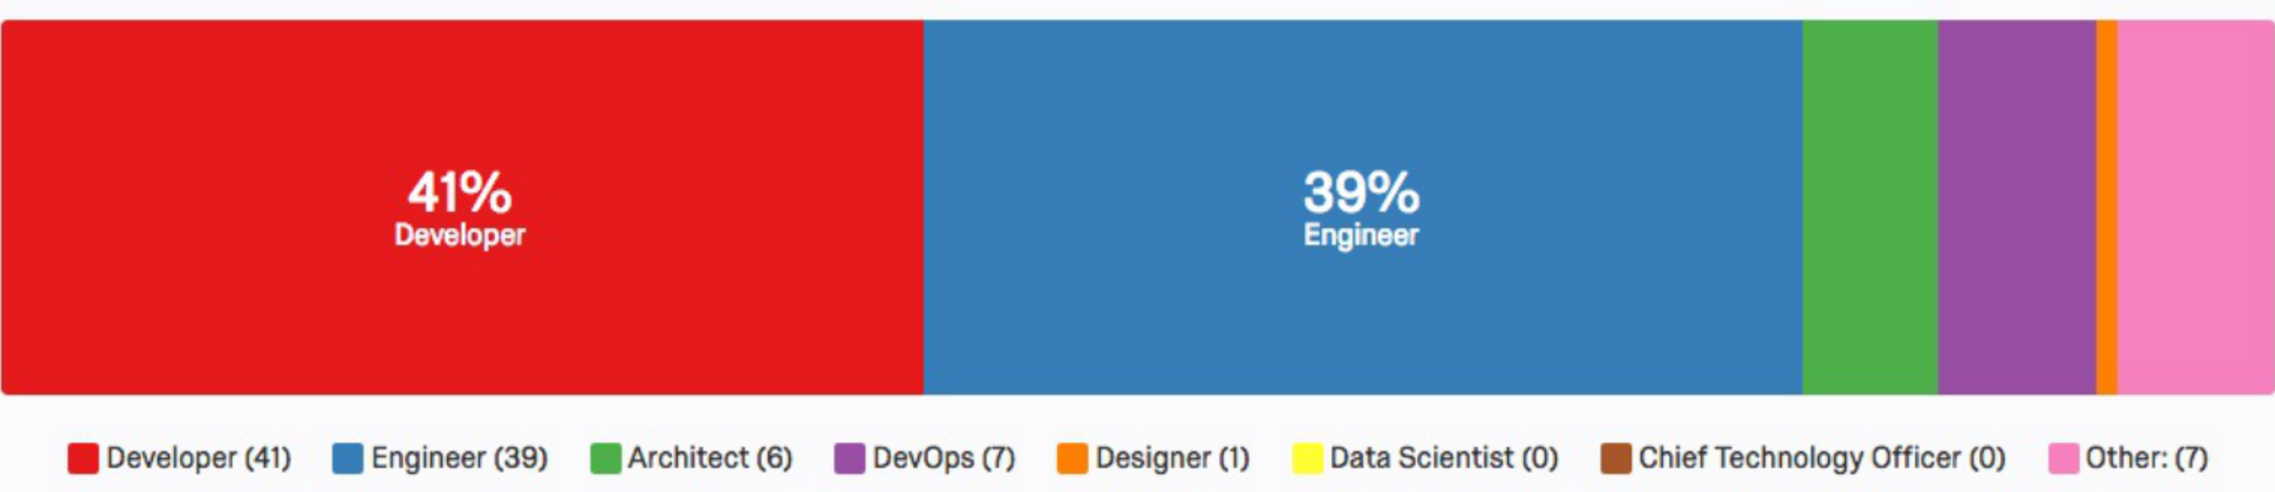
\includegraphics[width=1.105\textwidth,keepaspectratio]{ProcessesParticipantRoles}
\caption{Distribution of primary roles from Processes Survey~(S1) participants: 45.5\% are primarily a \textit{Developer}, 42.0\% an \textit{Engineer}, 12.5\% \textit{Other}, and 12.8\% were either \textit{DevOps}, \textit{Architect}, or \textit{Designer}. No participants selected \textit{Data Scientist} or \textit{Chief Technology Officer}.\vspace*{-0.3\baselineskip}}
\label{processes_roles}
\end{figure}

Survey participants had a mean of 9.1 years of programming experience, and primarily worked in teams of 2-5 members (45.10\% overall).
Participants were assumed to be software developers in some capacity, but primary roles within individual organizations can differ throughout the industry.
Participants were given seven different roles to select, as well as an \textit{Other} field to provide additional roles not included in the pre-populated options.
Figure~\ref{processes_roles} provides a visual illustration of the distribution of primary roles among participants.
87.5\% of participants were primarily a \textit{Developer} or \textit{Engineer} (45.5\% and 42.0\% respectively), with 6.9\% selecting \textit{DevOps}, 5.0\% \textit{Architect}, 1.0\% \textit{Designer}, and 12.5\% \textit{Other}.
Among participants that selected \textit{Other}, the open-text responses included: ``Tester,'' ``Security Analyst,'' ``Hobbyist Programmer,'' and ``Researcher.''

We divided the survey into four categories, with each containing 3-5 questions (see \cite{companion_site} for individual questions).
First, we elicited background information about demographics, roles, and experience.
Second, we asked questions relating to how and when developers become aware of merge conflicts.
Third, we asked questions related to planning and implementing merge conflict resolution strategies.
Finally, we asked questions about evaluating the effectiveness of those merge conflict resolutions and the particular tools that are used throughout the processes of working with merge conflicts.

\subsection{Barriers Survey (S2)}\label{perceptions_survey}

In the last step, we conducted a 50-question \textit{Barriers Survey} of software developers in order to examine the barriers, constraints, and concerns experienced when encountering merge conflicts.
We developed questions to confirm, extend, and broaden the results from the interviews.

\renewcommand*{\thefootnote}{\arabic{footnote}}
%\setcounter{footnote}{0}
We recruited participants for \textit{Barriers Survey}~(S2) to be similar to \textit{Processes Survey}~(S1) participants so that we could compare and triangulate the results.
We therefore recruited participants from contributor lists on popular open-source repositories on GitHub, advertised on social networking sites (Facebook, Twitter and Reddit), and by directly contacting software developers via email. 
Participants spanned a variety of organization structures and geographical locations, giving generalizability to results.
The survey was conducted online and anonymity was guaranteed in order to elicit honest responses from participants.
The \textit{Barriers Survey}~(S2) was available for 56 days and we received 162 survey responses, but individual parts of the survey have varying response rates and are reported where appropriate in Section~\ref{results}.

Survey participants were given six different software roles to select, and in many cases, participants considered themselves to be fulfilling multiple roles. 
Table~\ref{survey_roles} provides a pairwise breakdown of participants' role selections, with a majority of participants considering themselves to be \textit{Software Engineer/Developer} (95.1\% overall).
Survey participants indicated a median software development experience of 6-10 years (36.4\% overall), and worked on project sizes ranging from 2 to more than 51 developers (the median was 2-5 developers, constituting 48.8\% of all responses).

\vspace*{-0.8\baselineskip}

\begin{table}[!htbp]
\caption{Barriers Survey (S2) Participant Roles\textsuperscript{i}}
\label{survey_roles}
\centering
\begin{tabularx}{\textwidth}{@{}r|*{10}{C}c@{}}
\toprule
\addlinespace[4.5em]
	& \begin{rotate}{30} Soft. Developers \end{rotate} 
	& \begin{rotate}{30} Sys. Architects \end{rotate} 
	& \begin{rotate}{30} DevOps \end{rotate} 
	& \begin{rotate}{30} Project Managers \end{rotate}
	& \begin{rotate}{30} Project Maintainers \end{rotate}
	& \begin{rotate}{30} Sys. Admins \end{rotate}
	& \begin{rotate}{30} Other \end{rotate}\\
\midrule
	Software Developers & 154 & & & & & & \\
	System Architects & 53 & 54 & & & & & \\
	DevOps & 51 & 34 & 53 & & & & \\
	Project Managers & 44 & 29 & 20 & 44 & & & \\
	Project Maintainers & 39 & 21 & 24 & 22 & 40 & & \\
	Systems Administrators & 22 & 16 & 15 & 14 & 12 & 23 & \\
	Other & 8 & 4 & 4 & 3 & 1 & 2 & 11 \\
\bottomrule
	\multicolumn{8}{c}{\noindent\parbox[t]{11.7cm}{\vspace{0.4em}\textsuperscript{i}\hspace{0.2em}\textit{Barriers Survey}~(S2) participants were allowed to select multiple roles. Each entry represents the number of participants that selected both of the roles indicated for the column and row. 62 out of 162 participants (38\%) selected three or more roles.}\vspace*{-0.3\baselineskip}}
\end{tabularx}
\end{table}

We divided the \textit{Barriers Survey}~(S2) into four categories, each category containing 5-7 questions (see \cite{companion_site} for a list of questions).
First, we elicited background information about demographics, roles, and experience.
Second, we asked questions related to difficulties that developers experience when encountering merge conflicts.
Third, we asked questions related to conflict resolution and the factors that affect developers.
Finally we asked questions about the tools and tool features that developers use when working with merge conflicts.
Questions were presented either as 5-point Likert-type scales (with no pre-selected answers) or open-ended text forms to gather additional insights.

\subsection{Data Analysis}\label{analysis}
To ensure that our survey samples are representative of the larger developer population, we compare the demographics from the \textit{Processes Survey}~(S1) and the \textit{Barriers Survey}~(S2) with the results of the 2018 StackOverflow Developer Survey\footnote{https://insights.stackoverflow.com/survey/2018}.

The 2018 StackOverflow Developer Survey was conducted on 101,592 software developers from 183 countries.
This survey includes the number of years spent coding professionally by 77,903 participants.
%, and is presented as totals for buckets of 0-2 years, 3-5 years, 6-8 years, 9-11 years, 12-14 years, 15-17 years, 18-20 years, 21-23 years, 24-26 years, 27-29 years, and 30 or more years.
%For comparison purposes, we similarly grouped the results from the \textit{Processes Survey}~(S1) and the \textit{Barriers Survey}~(S2).
Figure~\ref{populations} provides a graphical representation of the percentile distribution of professional programming experience among participants in the \textit{Processes Survey}~(S1), \textit{Barriers Survey}~(S2), and the 2018 StackOverflow Developer Survey.
We see that our sample population has more experienced developers, and the trends match between all three samples.

\begin{figure}[!htbp]
\centering
\fbox{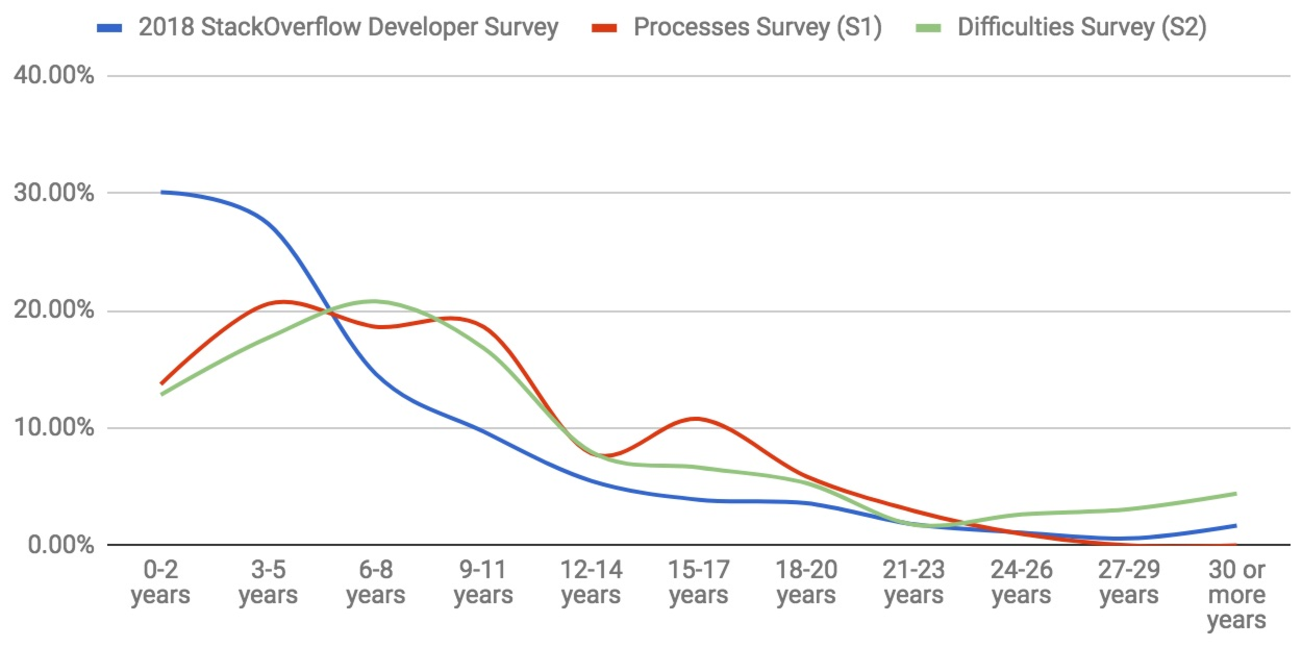
\includegraphics[width=0.98\textwidth,keepaspectratio]{imgs/populations}}
\caption{Percentile distributions of professional programming experience compared between \textit{Processes Survey}~(S1), \textit{Barriers Survey}~(S2), and 2018 StackOverflow Developer Survey participants. Responses are inclusively binned into 3-year buckets for comparison across surveys.\vspace*{-0.3\baselineskip}}
\label{populations}
\end{figure}

To further compare the distribution of programming experience across these population samples, we conduct nonparametric tests of the equality of the probability distributions between two samples.
Comparing \textit{Processes Survey}~(S1) responses with 2018 StackOverflow Developer Survey responses, we conclude that we cannot reject the null hypothesis that these samples were drawn from the same population distribution (Two-sample Kolmogorov-Smirnov test, $D = 0.33636$, p-value$ = 0.5939$).
We similarly conclude that \textit{Barriers Survey}~(S2) responses and 2018 StackOverflow Developer Survey responses could plausibly be drawn from the same population distribution (Two-sample Kolmogorov-Smirnov test, $D = 0.27273$, p-value$ = 0.8326$).
In both cases, we cannot reject the null hypothesis that the survey sample population is the same as the 2018 StackOverflow Developer Survey population, therefore, we conclude that our samples are representative of the development community.

\subsubsection{Interview Analysis}

Interviews were audio-taped and transcribed. 
The first and third authors unitized~\cite{unitization} the interview transcripts into cards that each contained a single logically consistent statement. 
To organize these cards we employed card sorting, a collaborative technique of exploring how people think about a certain topic~\cite{spencer2009card,card_sort}, which allows key concepts and associations to be identified through an open sorting method that iteratively develops categories during the process.

We performed two iterations of the open card sorting process.
In the first iteration, we developed a standardized coding scheme and improved it to an acceptable point through \textit{negotiated agreement,} which was reached when no further thematic categories could be created and agreed upon by both coders~\cite{garrison2006revisiting,ritchie2013qualitative}.
The coding scheme dictated that sentences must be consecutive and topically related to be grouped into a single card.
Logically connected statements that were separated by other lines were considered to be separate cards, as a conservative measure to preserve context within each card.

In the second iteration, the first and third authors sorted cards according to our coding scheme and discussed the resulting taxonomies until consensus was reached.
Based upon our research questions, we grouped the resulting categories as follows: the processes that developers use for merge conflicts (Section~\ref{RQ1}, the difficulties that developers face with merge conflicts (Section~\ref{RQ2}), and the impact of development tools on the resolution process (Section~\ref{RQ3}).

\subsubsection{Survey Analysis}

For the \textit{Processes Survey}~(S1), we evaluated the distribution of survey answers for each of the four Likert-type question by analyzing across demographic categories.
We used Likert-type questions to measure the extent to which participants agreed with a particular statement, or the degree to which a factor has impacted the participant.
Where answers differed across a demographic category, we note the difference and provide further discussion of these results.

The \textit{Processes Survey}~(S1) contained five open-ended questions.
We performed open thematic coding~\cite{fereday2006demonstrating} to analyze the responses to these questions.
The resulting codebook, including descriptions and examples, are available on our companion site~\cite{companion_site}.
%Table~\ref{tab:codes} provides the resulting codebook, including descriptions and examples.
After establishing a codebook, the first two authors independently coded the responses to each open-ended question.
For question 7 (\textit{``How do you monitor for merge conflicts?''}), we achieve an inter-rater reliability (IRR) agreement of $0.95$ (Jaccard similarity coefficient).
For questions 8 (\textit{``How do you determine the urgency of a merge conflict?''}), 11 (\textit{``What is your first step in trying to understand code involved in a merge conflict?''}), 14 (\textit{``What effect did deferring your response to a merge conflict have on the resolution of the conflict?''}), and 19 (\textit{``If your first attempt at resolving a merge conflict fails, what backup strategies do you use?''}), we achieve IRR agreements of $0.81$, $0.88$, $0.74$, and $0.92$, respectively (all are above the Software Engineering research standard of $0.80$ IRR).

%\def\shift{\hspace{0.5em}}
%\begin{table}[!htbp]
%\centering
%\caption{Codebook used for coding open-ended responses from Processes Survey (S1)}
%\label{tab:codes}
%\begin{tabular}{lp{1.5in}p{1.3in}}
%\toprule
%Code & Description & Example \\
%\midrule
%\multicolumn{3}{l}{\textbf{Q7: How do you monitor for merge conflicts?}} \\
%\shift Proactive & & \\
%\shift Reactive & & \\
%\midrule
%\multicolumn{3}{l}{\textbf{Q8: How do you determine the urgency of a merge conflict?}} \\
%\shift Project Structure & & \\
%\shift Code Under Conflict & & \\
%\shift External Dependencies & & \\
%\shift No System & & \\
%\midrule
%\multicolumn{3}{p{4.5in}}{\raggedright\textbf{Q11: What is your first step in trying to understand code involved in a merge conflict?}} \\
%\shift About the conflict & & \\
%\shift The Code Itself & & \\
%\shift Analyzing the code & & \\
%\shift Design Concerns & & \\
%\shift Project Organization & & \\
%\shift No-op & & \\
%\midrule
%\multicolumn{3}{p{4.5in}}{\raggedright\textbf{Q14: What effect did deferring your response to a merge conflict have on the resolution of the conflict?}} \\
%\shift Physical Manifestations & & \\
%\shift External to company impact & & \\
%\shift Policy/culture changes & & \\
%\shift The Nuclear Option & & \\
%\shift Increased Complexity & & \\
%\shift Stop the presses & & \\
%\shift No-op & & \\
%\midrule
%\multicolumn{3}{p{4.5in}}{\raggedright\textbf{Q19: If your first attempt at resolving a merge conflict fails, what backup strategies do you use?}} \\
%\shift Collaborating & & \\
%\shift Redoing changes & & \\
%\shift Take it offline & & \\
%\shift Try again & & \\
%\shift No strategy/Other & & \\
%\bottomrule
%\end{tabular}	
%\end{table}

We evaluated the results of the \textit{Barriers Survey}~(S2) by performing open card sorting on the all open-ended questions.
The resulting categories were standardized to an acceptable point through \textit{negotiated agreement}~\cite{ritchie2013qualitative}.

The \textit{Barriers Survey}~(S2) was primarily composed of Likert-type questions, which were used to measure the extent to which participants agreed with a particular statement.
This means that lower mean and median values indicate less agreement with the statement in a particular question.
We use this design to validate both the degree of agreement to the interview results, as well as the existence of individual factors.

We present the results of the \textit{Exploratory Interviews,} \textit{Processes Survey}~(S1) and \textit{Barriers Survey}~(S2) in Section~\ref{results}.
When necessary, we refer to individual survey participants by a combination of the survey short-hand (S1 or S2) and participant number; for example S1--14 is participant 14 from the \textit{Processes Survey}~(S1) responses.
\section{Results}\label{results}

\boldif{Results from interviews indicated that a common model of operating with merge conflicts exists.}
To understand how developers manage merge conflicts, we asked interview participants to describe their current processes for handling merge conflicts.

\boldif{\textit{Add anecdotal quotes and descriptions from interviews to highlight these observations.}}
Participants talked about different steps that they follow, including using tools that alert them to potential or current merge conflicts, processes for analyzing and understanding conflicting code prior to implementing a resolution, and the use of tools for validating that their resolution worked.
As an example, P3 said:
\begin{quoting}
\textit{``Part of my job on the integration team requires that I check for bad regressions. I use scripts to track patches as they're being backported, so I know when and where to look if [a patch] introduces a conflict. [\ldots] And once I've fixed [the conflict], I try to compare with the previous version to make sure [the code] works in a similar way.''}
\end{quoting}

\boldif{Provide descriptions that link the stages of Merge Conflict model to this quote. Use it to drive description of simplified model description paragraph}

\boldif{Based on these anecdotal observations, we construct an initial model of the processes that developers employ when working with merge conflicts, see Fig.~\ref{model}.}
Our interview and survey results suggest that developers follow a series of phases through which they manage the life-cycle of individual merge conflicts.
We construct a model of the developer processes for managing merge conflicts and examine each phase in detail.
Figure~\ref{model} provides an illustration of this model. 
It consists of four phases: \emph{awareness, planning, resolution,} and \emph{evaluation.}

\boldif{Discuss the fact that no other studies have shown that a model exists for merge conflicts}

\begin{figure}[!htbp]
\centering
\fbox{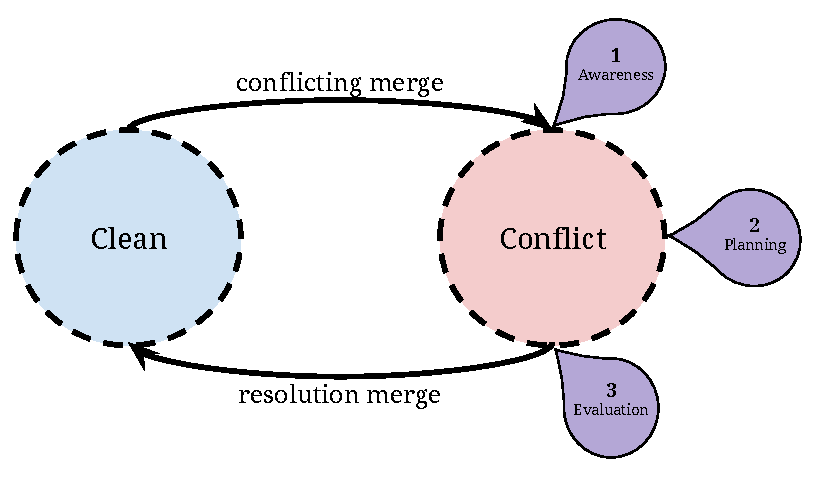
\includegraphics[width=0.90\textwidth,keepaspectratio]{imgs/MergeConflictModel}}
\caption{Model of Developer Processes for Managing Merge Conflicts. Developers alternate between \textit{clean} and \textit{conflicting} states of code. Beginning from (1)~\textit{development}, developers maintain (2)~\textit{awareness} of conflicts within the codebase in different ways. Once aware, developers begin (3)~\textit{planning} for a (4)~\textit{resolution} to fix the conflict. And finally, developers (5)~\textit{evaluate} the effectiveness of their deployed resolutions (returning to \emph{planning} if the resolution failed).\vspace*{-0.3\baselineskip}}
\label{model}
\end{figure}

\boldif{Awareness is how developers become aware}
First, the \emph{awareness} phase consists of the actions developers take to become aware of merge conflicts.
This could be passive, as the developer will become aware of a merge conflict when attempting to merge changes or perform a pull.
At the other end of the spectrum are developers who \emph{proactively} monitor for merge conflicts as they write code.
They are actively looking for changes that might be problematic, either manually or through the use of specialized tools.

\boldif{Planning is when developers plan their future actions}
Second, the \emph{planning} phase occurs after the developer has become aware that a conflict has occurred, and they are about to tackle the conflict.
This includes the decision of when they will try and resolve the conflict.
Some developers might try and resolve it immediately, while others might postpone the resolution.
Some might change their strategy depending on the conflict, incoming deadlines, or availability of resources.
This also includes other actions, such as if they are going to tackle the conflict alone, or collaborate with other developers knowledgeable in the area of conflict~\cite{CostaSarma}.

\boldif{Resolution is the action of implementing a resolution. Mundane and well understood, so we focus on the other three.}
Third, the \emph{resolution} phase represents the implementation of the planned resolution.
Several tools exist that help in this phase~\cite{nishimura,mens2002state,Brun2011}.
Here we focus on the difficulties that developers face during these resolution implementations (see Section~\ref{RQ2}).

\boldif{Evaluation is how developers check that their solution is correct}
Finally, after the conflict has been resolved, developers enter in the \emph{evaluation} phase.
In this phase, the developer has to evaluate their resolution before considering the conflict as resolved.
This is to ensure the correctness of the resulting code.
Possible actions during this stage includes compiling the source code.
Developers wanting more guarantees can go a step further and run the tests.
Finally, some groups have policies such as code reviews that need to be performed on the merge conflict resolution.
 
\boldif{To explore and validate this model, we asked developers to reflect upon how they become aware of merge conflicts, how they plan for merge conflict resolutions, and how they evaluate their resolutions in the \textit{Processes Survey}.}
In order to explore and validate this model, and our assumptions, we conducted the \emph{Processes Survey}.
Our aim in this survey was to understand how developers become aware of merge conflicts (what steps they take, what tools they use, etc.).
Also, we wanted to investigate their strategies for dealing with merge conflicts and how they decide whether the resolution has addressed all of their concerns.

Results are categorized according to the life-cycle of merge conflicts; with specific results for the \textit{awareness} (Section~\ref{RQ1}), \textit{planning} (Section~\ref{RQ2}), and \textit{evaluation} phases (Section~\ref{RQ3}).
We then present the difficulties that developers experience when managing merge conflicts (Section~\ref{RQ4}).
And finally, we examine the gaps in tool support for managing merge conflicts according to developer's needs (Section~\ref{RQ5}).
%!TEX root = main.tex

\subsection{\textbf{RQ1:} Ho do software developers manage merge conflicts?}\label{RQ1}

\boldif{Results from interviews indicated that a common model of operating with merge conflicts exists.}
To understand how developers manage merge conflicts, we asked interview participants to describe their current processes for handling merge conflict.

\boldif{\textit{Add anecdotal quotes and descriptions from interviews to highlight these observations.}}
Participants talked about different steps that they follow, including using tools that alert them to potential or current merge conflicts, processes for analyzing and understanding conflicting code prior to implementing a resolution, and the use of tools for validating that their resolution worked.
As an example, P3 said:
\begin{quoting}
\textit{``Part of my job on the integration team requires that I check for bad regressions. I use scripts to track patches as they're being backported, so I know when and where to look if [a patch] introduces a conflict. [\ldots] And once I've fixed [the conflict], I try to compare with the previous version to make sure [the code] works in a similar way.''}
\end{quoting}

\boldif{Provide descriptions that link the stages of Merge Conflict model to this quote. Use it to drive description of simplified model description paragraph}

\boldif{Based on these anecdotal observations, we construct an initial model of the processes that developers employ when working with merge conflicts, see Fig.~\ref{model}.}
Our interview and survey results suggest that developers follow a series of phases through which they manage the life-cycle of individual merge conflicts.
We construct a model of the developer processes for managing merge conflicts and examine each phase in detail.
Figure~\ref{model} provides an illustration of this model. 
It consists of four phases: \emph{awareness, planning, resolution,} and \emph{evaluation.}

\boldif{Discuss the fact that no other studies have shown that a model exists for merge conflicts}

\begin{figure}[!htbp]
\centering
\fbox{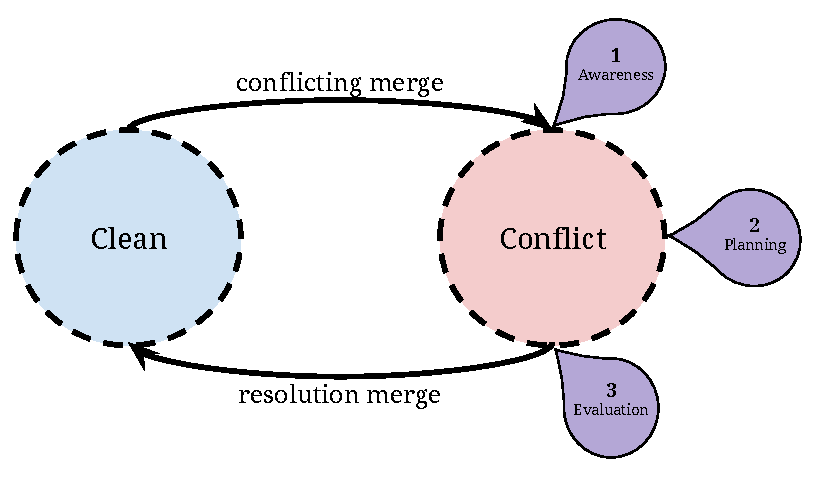
\includegraphics[width=0.90\textwidth,keepaspectratio]{imgs/MergeConflictModel}}
\caption{Model of Developer Processes for Managing Merge Conflicts. Developers alternate between \textit{clean} and \textit{conflicting} states of code. Beginning from (1)~\textit{development}, developers maintain (2)~\textit{awareness} of conflicts within the codebase in different ways. Once aware, developers begin (3)~\textit{planning} for a (4)~\textit{resolution} to fix the conflict. And finally, developers (5)~\textit{evaluate} the effectiveness of their deployed resolutions (returning to \emph{planning} if the resolution failed).\vspace*{-0.3\baselineskip}}
\label{model}
\end{figure}

\boldif{Awareness is how developers become aware}
First, the \emph{awareness} phase consists of the actions developers take to become aware of merge conflicts.
This could be passive, as the developer will become aware of a merge conflict when attempting to merge changes or perform a pull.
At the other end of the spectrum are developers who \emph{proactively} monitor for merge conflicts as they write code.
They are actively looking for changes that might be problematic, either manually or through the use of specialized tools.

\boldif{Planning is when developers plan their future actions}
Second, the \emph{planning} phase occurs after the developer has become aware that a conflict has occurred, and they are about to tackle the conflict.
This includes the decision of when they will try and resolve the conflict.
Some developers might try and resolve it immediately, while others might postpone the resolution.
Some might change their strategy depending on the conflict, incoming deadlines, or availability of resources.
This also includes other actions, such as if they are going to tackle the conflict alone, or collaborate with other developers knowledgeable in the area of conflict~\cite{CostaSarma}.

\boldif{Resolution is the action of implementing a resolution. Mundane and well understood, so we focus on the other three.}
Third, the \emph{resolution} phase represents the implementation of the planned resolution.
Several tools exist that help in this phase~\cite{nishimura,mens2002state,Brun2011}.
Here we focus on the difficulties that developers face during these resolution implementations (see Section~\ref{RQ2}).

\boldif{Evaluation is how developers check that their solution is correct}
Finally, after the conflict has been resolved, developers enter in the \emph{evaluation} phase.
In this phase, the developer has to evaluate their resolution before considering the conflict as resolved.
This is to ensure the correctness of the resulting code.
Possible actions during this stage includes compiling the source code.
Developers wanting more guarantees can go a step further and run the tests.
Finally, some groups have policies such as code reviews that need to be performed on the merge conflict resolution.
 
\boldif{To explore and validate this model, we asked developers to reflect upon how they become aware of merge conflicts, how they plan for merge conflict resolutions, and how they evaluate their resolutions in the \textit{Processes Survey}~(S1).}
In order to explore and validate this model, and our assumptions, we conducted the \emph{Processes Survey}~(S1).
Our aim in this survey was to understand how developers become aware of merge conflicts (what steps they take, what tools they use, etc.).
Also, we wanted to investigate their strategies for dealing with merge conflicts and how they decide whether the resolution has addressed all of their concerns.

\boldif{We present the results to these research questions in Sections~\ref{RQ1a}, \ref{RQ1b}, and \ref{RQ1c}.}
Sections~\ref{RQ1a}, \ref{RQ1b}, and \ref{RQ1c} presents the results to these research questions.

\subsubsection{\textbf{RQ1a:} How do software developers become \textbf{aware} of merge conflicts?}\label{RQ1a}

\boldif{Developers use 2 methods for becoming aware of merge conflicts: proactive and reactive.}
From the \textit{Processes Survey}~(S1) we found that 29.41\% of participants do not actively monitor for merge conflicts during their development activities.
For the rest of the developers who answered with \emph{yes} or \emph{sometimes} (61.77\%), we identified 61 different tools mentioned in 126 instances.

\nsubsection{Reactive and Proactive Monitoring for Merge Conflicts}

\boldif{Reactive detection only notifies developers that a merge conflict \emph{has happened}. Developers use it to minimize the size/complexity of the conflict, or it's impact on the team.}
Reactive monitoring for merge conflicts notifies the developer that a conflict has already occurred.
However, developers still use this process to manage or reduce the complexity of a conflict.
For the developers who answered that they monitor for merge conflicts (replied either \emph{yes} or \emph{sometimes}), we found that 73.68\% (42 out of 57 responses; 6 participants left this field blank) described reactive processes.
For example, participant S1--48 said they use integration tools to detect merge problems before they advance to testing:
\begin{quotation}
	[\ldots] integration tests tell us if builds are breaking and we use those to locate merge conflicts. [\ldots] we use it to catch merge bugs before they go to smoke testing for release
\end{quotation}
And participant S1--64 mentioned that they try to solve merge conflicts early in order to minimize disruptions to the team:
\begin{quotation}
	We try to catch conflicts early so that fewer developers have to be involved in looking at broken code.
\end{quotation}

\boldif{Proactive monitoring allows devs to detect MC before they happen. However, it is more involved, as it requires a lot more manual effort from the developers.}
Proactive monitoring allows developers to preemptively catch merge conflicts before they happen.
15 participants (14.71\%) mentioned they achieved this by manually tracking incoming changes, such as participant S1--35 who indicated:
\begin{quotation}
	I monitor commit logs before I begin merging branches so that I see any potentially overlapping code that will break the merge.
\end{quotation}
Other teams rely more on communication.
This can happen during regular team meetings, to make sure that everybody is aware of each other's tasks, for example participant S1--46 said:
\begin{quotation}
	[\ldots] standups allow us to know where everyone is working that week.
\end{quotation}
While 10 participants (9.80\%) indicated that they broadcast their changes in order to notify team members if they will make breaking changes.
For example, participant S1--102 indicated that team members:
\begin{quotation}
	[\ldots] send emails before making breaking changes to the API or related sub-modules.
\end{quotation}

\boldif{Developers do not regularly actively monitor for merge conflicts. ...}
To conclude, only a third of developers actively monitor for merge conflicts.
When developers are caught unaware of the conflict, they are more likely to be interrupted by it.
This can lead to more frustration, as they do not have any warning of when the conflict will occur and whether they have the time to deal with it immediately.

\nsubsection{Tools for Monitoring for Merge Conflicts}

\boldif{The tools that developers use allow for only a \emph{reactive} approach.}
Examining the tools used by participants with reactive processes, we find that 87.72\% of these participants rely on version control systems (e.g. Git, SVN, TFS, CVS), while 21.05\% use continuous integration systems (e.g. Jenkins, Travis CI, TeamCity).
Table~\ref{s1_toolset} presents the top 10 tools developers use when monitoring for merge conflicts, including the totals for both reactive and proactive strategies.

Additionally, we examine the tools used by participants with proactive processes.
We find that all participants with a proactive strategy rely on version control systems, and 33.33\% use continuous integration systems.
Additionally, 26.66\% of proactive participants use code analysis tools (e.g. SonarQube, Code Climate).

We find that the majority of tools used by developers for merge conflict monitoring are built to only support reactive strategies, and that multiple tools must be used in conjunction for a proactive approach.

%\boldif{Devs do not use existing workspace awareness tools that come from the acadmemia.}
%When collaborating, developers generally rely on passive communication tools, like email, to coordinate.
%Developers are currently not leveraging the functionalities provided by many research prototypes (e.g., Palant\'{i}r~\cite{palantir}, Crystal~\cite{Brun2011}) that are specifically designed to facilitate proactive conflict detection.

\begin{table}[!htbp]
\renewcommand{\arraystretch}{1.3}
\caption{Merge Awareness Toolsets (Top 10) from Processes Survey (S1)}
\label{s1_toolset}
\centering
\begin{tabularx}{\textwidth}{ll|cc|c}
\toprule
% \textbf{Par.}\parnote{Par. = Total number of survey participants using each tool.}
% \vspace*{-0.3\baselineskip}
  \parnoteclear % tabularx will otherwise add each note thrice
  Tool\parnote{\textit{Processes Survey}~(S1) participants were allowed to provide multiple tools. 57 out of 102 participants (56\%) indicated the use of at least one merge awareness tool.} & Description & Proactive\parnote{Participants using this tool with a proactive strategy.} & Reactive\parnote{Participants using this tool with reactive strategy.} & Total\parnote{Total number of survey participants using each particular tool.}\\
\midrule
  Git & Version Control System & 10 & 30 & 40\\
  Email (unspecified) & Email Client or System & 2 & 4 & 6\\
  GitHub & Project Hosting Site & 2 & 5 & 7\\
  SVN & Version Control System & 0 & 4 & 4\\
  Visual Studio & IDE & 1 & 2 & 3\\
  PagerDuty & IT Incident Manag. Sys. & 0 & 3 & 3\\
  GitLab & Project Hosting Site & 2 & 1 & 3\\
  Jenkins & Continuous Integration & 0 & 3 & 3\\
  VCS (unspecified) & Version Control System & 2 & 2 & 4\\
  Team Foundation Server & Version Control System & 1 & 1 & 2\\
\bottomrule
\end{tabularx}
\parnotes
\end{table}


\boldif{Therefore their approaches are mostly \emph{reactive,} and their tool selection reflects that.}
To summarize, we find that developers employ \emph{reactive} processes, even if they are proactive in monitoring for merge conflicts once they have occurred.
This can be seen as a consequence of the tools that developers have at their disposal.
All the tools mentioned support only a \emph{reactive} approach, which biases developers towards one particular solution.
If developers want a more \emph{proactive} approach, then based on the tools they use, they need to come up with their own solution.
The most often cited techniques involve increasing communication among developers.
While this technique might be effective in small teams, it scales very poorly and cannot be effectively used in larger organizations~\cite{brooks1974mythical}.

\boldif{All the above point towards a need for better collaborative tools, that promote a proactive approach}
Finally, our results point to the conclusion that developers are not aware of existing proactive tools (e.g. Palant\'{i}r~\cite{sarma_palantir:_2003}, Crystal~\cite{Brun2011}), and are therefore not leveraging those tools to actively monitor for merge conflicts.
However, developers are trying to mitigate the severity of merge conflicts by attempting to resolve them as soon as they become aware.

\subsubsection{\textbf{RQ1b:} How do software developers \textbf{plan} for merge conflict resolutions?}\label{RQ1b}

\boldif{Developers use different strategies for dealing with MC}
When encountering a merge conflict, developers follow different strategies.
They can either: (a) defer the merge conflict to a later date, or; (b) solve the conflict.
In the \textit{Processes Survey}~(S1) we sought an understanding of these strategies and when developers use them.
The tools that developers use when implementing merge conflict resolutions are discussed in Section~\ref{RQ3}.

\nsubsection{Deferring Responses to Merge Conflicts}

\boldif{25\% of developers consider all conflicts as being equally urgent.}
One quarter of our participants consider all merge conflicts to be equally urgent.
This means that they will always solve the conflict as soon as the 
We can assume that most developers will interrupt their work regardless of the type of merge conflict.
Therefore, they will give the same level of attention, for example, to a conflict generated by whitespace or formatting changes, as a conflict that is generated by overlapping logical changes. 
%TODO: Make sure this fits in the flow.

\boldif{The first option is that they might defer the MC, for a later time}
The easiest option when encountering a merge conflict is to simply not deal with it.
Indeed, we found that 56.18\% of participants have deferred at least once when responding to a merge conflict.
The reasons for deferring are varied and listed in Table~\ref{s1_deferring_response}.

The location and complexity of conflicting code (D1, D2) were the most selected factors, and match the top difficulty factors of merge conflicts (F1, F2) as described in Section~\ref{difficulty-factors}.
% TODO Add a conclusion statement about the meaning of these factors being top in both tables.

As the third most selected factor, \textit{ownership of the conflicting code}~(D3) indicates that the deferral is not always temporal, but can also be logistical when developers defer to other team members.
Participant S1--8 succinctly defines the role ownership impacts his workflow as:
\begin{quotation}
	Code is mine? I fix it. Code is others? I submit PR or bug reports.
\end{quotation}
We additionally asked participants to rate the degree to which code ownership factors into their overall merge conflict strategy, and participants indicate that code ownership factors \textit{about half the time} in their strategy of code ownership (mean: $3.21$ on a 5-point Likert-type scale).
Only 10.11\% of participants indicated that code ownership \textit{never} factors into their resolution strategy.

\begin{table}[!htbp]
\renewcommand{\arraystretch}{1.2}
\caption{Factors in Deferring Responses to Merge Conflicts from Processes Survey (S1)}
\label{s1_deferring_response}
\centering
\begin{tabularx}{\textwidth}{>{\rowmac}c | >{\rowmac}l | >{\rowmac}c | >{\rowmac}r <{\clearrow}}
\toprule
  \parnoteclear % tabularx will otherwise add each note thrice
  Factor & Description & \# Selections\parnote{\textit{Processes Survey}~(S1) participants were allowed to select multiple factors. 44 out of 102 participants (43\%) selected more than one factor.\vspace*{-0.9\baselineskip}} & Percentage (\%)\textsuperscript{i} \\
\midrule
  D1 & Complexity of the conflicting code & 36 & 25.00\% \\
  D2 & Number of conflicting code locations & 32 & 22.22\% \\
  D3 & Ownership of the conflicting code & 25 & 17.36\% \\
  D4 & Size of the conflicting code & 20 & 13.89\% \\
  D5 & Approaching deadlines & 13 & 9.03\% \\
  D6 & Work schedule constraints & 2 & 1.39\% \\
  D7 & Other\hspace{4.6cm} & 7 & 4.86\% \\
\bottomrule
\end{tabularx}
\parnotes
\end{table}

\boldif{60\% of developers defer a merge conflict, at least once. However, there doesn't seem to be a systematic understanding of the effect of such a deferral.}
%Our study results indicate that 60\% of developers have deferred a merge conflict at least once. 
While developers have listed multiple reasons for deferral, two stand out: complexity and the number of conflicting locations.
Both of these reasons indicate that a developer is more likely to defer if the conflict resolution appears to be lengthy, either because the potential changes are non-trivial or because there are many smaller conflicts requiring the developers' attention.

\nsubsection{Deferring Response to Merge Conflicts}

\boldif{Deferring can have bad consequences, including increased complexity and delaying features. Organizations have sometimes changed the policy to prevent this.}
Deferring the merge conflict resolution comes with a price.
Table~\ref{effects-deferral} shows the top effects of deferring a response to a merge conflict.
The most common effect was that developers have had to stop the development (\emph{Stop the Presses,} 15 responses) in order to resolve the conflicts.
This halt in development includes asking team members to also refrain from adding any additional code into the codebase.
The second most common effect is the \textit{increased complexity} of the conflicts (E2), reported by nine participants.
Participant S1--93 noted that:
\begin{quotation}
	Deferring a merge conflict simply kicks the can down the road (or off a cliff). Typically resolving the conflict only gets more difficult as time passes.
\end{quotation}
Participant S1--70 even hinted that the increased complexity can be quite severe, on an order of magnitude greater than if the conflict were addressed immediately:
\begin{quotation}
	Untangling takes days instead of minutes when it gets too out of hand.
\end{quotation}
In some cases, features had to be removed from releases, in order for integration problems to be mitigated and the conflict to be successfully resolved. S1--5 said:
\begin{quotation}
	We have had several releases come up short in new features because they got delayed by integration problems.
\end{quotation}
Finally, in order to prevent similar problems arising, some organizations have instituted \textit{policy changes} (E4) to prevent this from happening in the future. Participant S1--46 said:
\begin{quotation}
	We've had devs push a bunch of code up before going on holiday and mucking up a release, so we've instituted an all hands on deck policy for the 2 weeks leading up to a major release
\end{quotation}

\boldif{However, some effect can be severe, including impact to customers, or having to reimplement features.}
In one extreme case, participant S1--9 reported that an unresolved merge conflict affected production software (E7), which resulted in downtime of the product, as it broke functionality:
\begin{quotation}
	Broke the app for customers until we could get a patch pushed [\ldots].
\end{quotation}
Finally, the merge conflicts can get too severe and intractable for developers to cope with the complexities.
In these types of situations, developers have to resort to the \emph{Nuclear Option} (E5), where they scrap their changes and manually reimplement them.
Such as in the case of S1--102, who said:
\begin{quotation}
	Uh.... KABOOM! More changes came in and everything piled up. Nothing to do but wipe it all back to clean and start trying to piece things back together.
\end{quotation}

\begin{table}[!htbp]
\renewcommand{\arraystretch}{1.2}
\caption{Effects of Deferring Response to a Merge Conflict from Processes Survey (S1)}
\label{effects-deferral}
\centering
\begin{tabularx}{\textwidth}{>{\rowmac}c | >{\rowmac}l | >{\rowmac}c | >{\rowmac}r <{\clearrow}}
\toprule
  \parnoteclear % tabularx will otherwise add each note thrice
  Effect & Description & \# Participants\parnote{46 out of 102 participants (45.1\%) provided a description of the effects of deferring.\vspace*{-0.8\baselineskip}} & Percentage (\%)\textsuperscript{i} \\
\midrule
  E1 & Stop the Presses & 15 & 32.61\% \\
  E2 & Increased complexity & 9 & 19.57\% \\
  E3 & Non-operation effects & 5 & 10.87\% \\
  E4 & Policy/cultural changes & 3 & 6.52\% \\
  E5 & The Nuclear Option & 2 & 4.35\% \\
  E6 & Physical manifestations & 1 & 2.17\% \\
  E7 & Impact beyond the organization \hspace{1cm} & 2 & 2.17\% \\
\bottomrule
\end{tabularx}
\parnotes
\end{table}
\vspace{0.8em}

\boldif{The results of such a deferral can be disastrous. However, it is difficult to make an assessment of the effect of the deferral when the decision to defer is being made.} 
The results of deferring can be disastrous. 
%Participants reported having to throw away code (the \emph{Nuclear Option}) and even rising to the level of customers and users experiencing broken functionality and loss of access.
However, it is difficult to assess a deferral to determine if it will turn a single merge conflict into a larger problem.
Tools could provide such information; responding to developers with enough information to make accurate and informed decisions in order to prevent further issues down the line.

\nsubsection{Attempting Resolution \& Initial Strategies}

\boldif{If they have not deferred, they need to understand the (changes in the) conflict}
When developers don't defer their response, they have to resolve the conflicts now.
They primarily approach merge conflicts by \textit{examining the merge} (U1), \textit{analyzing or manipulating the code} (U2), or \textit{examining the code} (U3).
Table~\ref{s1_understanding_code} lists all six strategies described by the \textit{Processes Survey}~(S1) participants.

\begin{table}[!htbp]
\renewcommand{\arraystretch}{1.2}
\caption{Initial Strategies for Understanding Conflicting Code from Processes Survey (S1)}
\label{s1_understanding_code}
\centering
\begin{tabularx}{\textwidth}{>{\rowmac}c | >{\rowmac}l | >{\rowmac}c | >{\rowmac}r <{\clearrow}}
\toprule
  \parnoteclear % tabularx will otherwise add each note thrice
  Strategy & Description & \# Participants\parnote{79 out of 102 participants (77\%) provided a description of their initial strategy.\vspace*{-0.3\baselineskip}} & Percentage (\%)\textsuperscript{i} \\
\midrule
  U1 & Examining the merge & 26 & 32.91\% \\
  U2 & Analysis/manipulation of the code & 19 & 24.05\% \\
  U3 & Examining the code & 18 & 22.79\% \\
  U4 & Focus on design concerns & 8 & 10.13\% \\
  U5 & Examine project organization & 6 & 7.60\% \\
  U6 & No strategy\hspace{3.5cm} & 2 & 2.53\% \\
\bottomrule
\end{tabularx}
\parnotes
\end{table}
\vspace{0.8em}

\boldif{The most common strategies for understanding the conflict are examining the conflict and analysis/manipulation of the code.}
Participant S1--44 described their strategy of \textit{examining the merge}~(U1) as:
\begin{quotation}
	Reviewing the most recent commits (comments and code) to see whether it's a shallow conflict or not.
\end{quotation}
	And participant S1--69 indicated their strategy of analyzing the code (U2) involves:
\begin{quotation}
[\ldots] determining if the merge conflict involves important functionality; stepping through with a debugger helps.
\end{quotation}
Overall, we find that developers initially focus on the code involved in the merge conflict or information related to the merge itself.

\boldif{Surprisingly, some developers do not have a strategy for MCR}
Surprisingly, we found that two of our participants (2.53\% of participants) indicated that they \textit{``don't have a strategy''} or \textit{``mostly try to fix it as soon as possible.''}

%\begin{figure}[!htbp]
%\centering
%\fbox{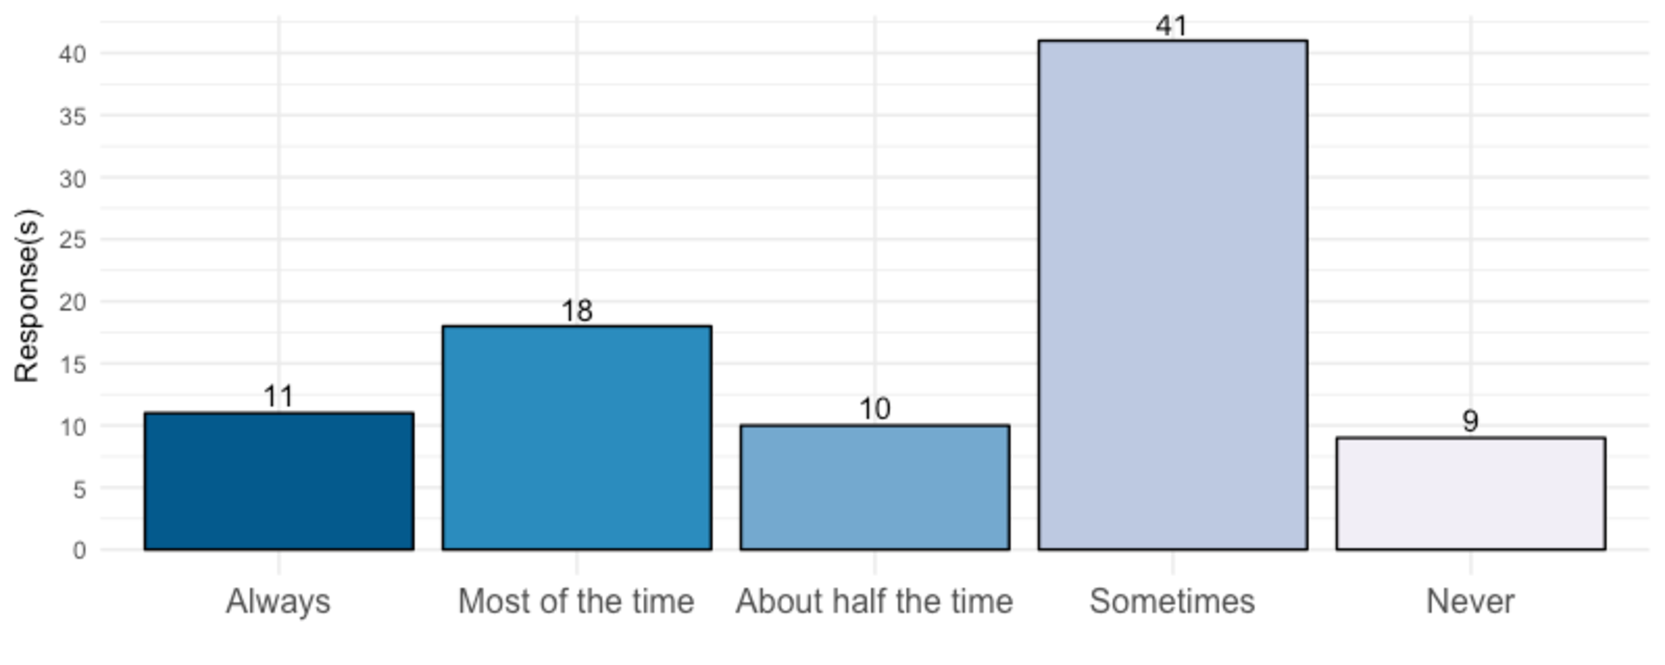
\includegraphics[width=0.98\textwidth,keepaspectratio]{imgs/CodeOwnershipFactor}}
%\caption{Degree of Code Ownership as a Factor in Merge Conflict Strategies. Scale: 1 is \textit{Always} and 5 is \textit{Never}. 89 out of 102 participants (87.26\%) provided a response to this question in the \textit{Processes Survey}~(S1).\vspace*{-0.3\baselineskip}}
%\label{fig:code-ownership-resolution}
%\end{figure}

To conclude, developers reported that expertise in the area of the conflicting code is one of the top factors in determining the difficulty of a merge conflict.
Additionally, developers also indicate that increases in perceived complexity of merge conflicts is strongly linked with the degree of difficulty in resolving them.
Therefore, developers' perceptions and intuition are relied on throughout the implementation of their resolution.

\nsubsection{Code Ownership in Merge Conflict Resolution Strategies}

\boldif{The role of code ownership in the resolution strategy.}
Finally, we found that, on average, participants indicate that code ownership factors \textit{about half the time} in their strategy of code ownership (mean: $3.21$ on a 5-point Likert-type scale).
This is consistent with their responses for their criteria for deferring a resolution, where it is the third most common factor in their decision. 
Only 10.11\% of participants indicated that code ownership \textit{never} factors into their resolution strategy (see Figure~\ref{fig:code-ownership-resolution}).

\subsubsection{\textbf{RQ1c}: How do software developers \textbf{evaluate} merge conflict resolutions?}\label{RQ1c}

After implementing a merge conflict resolution, software developers must evaluate whether their resolution has returned the codebase to a clean state.
We asked developers to select the conditions (from interviews) that they use to determine whether their resolution has successfully addressed the merge conflict.

\nsubsection{Success Conditions for Merge Conflict Resolutions}

In the \textit{Exploratory Interviews}, developers described six common conditions they considered important in their evaluation.
We asked \textit{Processes Survey}~(S1) participants to select from this list of conditions, including an \textit{Other} option to elicit additional conditions.
Only two developers selected that condition, indicating ``performance tests showing similar performance'' and ``client approval.''
We received 324 selections from 89 participants and present the aggregated results in Table~\ref{conditionsSuccess}.

\begin{table}[!htbp]
\caption{Conditions of Successful Merge Conflict Resolutions from Processes Survey (S1)\textsuperscript{i}}
\label{conditionsSuccess}
\centering
\begin{tabularx}{\textwidth}{@{}lr|*{7}{C}c@{}}
\toprule
	&
	& C1
	& C2
	& C3
	& C4
	& C5
	& C6
	& C7 \\
\midrule
	C1 & All tests pass & \textbf{67} & & & & & & \\
	C2 & Code compiles & 50 & \textbf{67} & & & & & \\
	C3 & Code looks correct & 50 & 54 & \textbf{66} & & & & \\
	C4 & VCS warmings gone & 38 & 42 & 41 & 51 & & & \\
	C5 & Code reviewed & 32 & 31 & 27 & 25 & 38 & & \\
	C6 & Merged to production & 27 & 27 & 27 & 26 & 19 & 33 & \\
	C7 & Other & 2 & 2 & 0 & 0 & 0 & 0 & 2 \\
\bottomrule
    \multicolumn{9}{c}{\noindent\parbox[t]{11.7cm}{\vspace{0.4em}\textsuperscript{i}\hspace{0.2em}\textit{Processes Survey}~(S1) participants were allowed to select multiple conditions. Each entry represents the number of participants that selected both of the conditions indicated for the column and row. 68 out of 102 participants (67\%) selected three or more conditions.}\vspace*{-0.3\baselineskip}} \\
\end{tabularx}
\end{table}

\textit{All tests pass} (C1), \textit{code successfully compiles} (C2), and \textit{code looks correct (i.e. visual test passes)} (C3) were the most commonly selected conditions required for a successful merge resolution.
These results are in line with existing literature showing that testing (C1) can be used for validating program functionality and correctness~\cite{beizer1984software,tian2005software}. %and have been fundamental to development processes such as test-driven development for several years~\cite{beck2003test}.
Similarly, the use of compilers to validate code (C2) as being executable and in good-working order will be familiar to any developer using a compiled programming language.

The use of visual inspection as a measure of successful merge conflict resolutions is surprising to us, given that \textit{complexity of conflicting lines of code}~(F1) is the highest rate factor for impact on merge conflict difficulty~\cite{mckee2017software}.
Inspecting code requires time and expertise in the area of conflicting code.
However, the survey participants that selected \textit{code looks correct (i.e. visual test passes)}~(C3) had a mean of 9.2 years of programming experience, which is only slightly higher than the overall mean of 9.0 years of programming experience.

Looking at the combination of \textit{code looks correct (i.e. visual test passes)}~(C3) with the other conditions, we find that 54 participants also selected \textit{all tests pass}~(C1) (52.9\%).
As the most common co-occuring selections, we conclude that although developers rely upon their expertise to visually inspect a merge conflict resolution, they also run the test suite to validate their evaluation.
Experience can play a big factor, as this method (C3) is highly subjective.

\boldif{Tests are still the most common criteria for determining a merge conflict resolution successful.}
The two most common evaluation criteria that developers mentioned are that the \emph{code compiles,} and that \emph{all tests pass.}
However, less then half selected both options.
While tests passing can be considered a good criteria of a successful resolution, the fact that the code compiles is not.
Even if the code compiles, there can be logical errors that are introduced during the merge resolution process, especially if the resolution was difficult.

\boldif{Only a minority of developers mention that code review is part of their success criteria}
Interestingly, only a minority of developers (37.25\%) mentioned code reviews as part of their success criteria.
%TODO add citation for the code review part
While code reviews are an effective way to detect bugs introduced by changes in the codebase, the practice appears to have not been adopted for code changed during merge conflict resolutions.

\nsubsection{Merge Resolution Evaluation Toolsets}

From the \textit{Exploratory Interviews}, we identified five categories of software development tools that developers mention in relation to merge conflicts.
In the \textit{Processes Survey}~(S1), we asked the developers to identify the tools they use when evaluating a merge conflict resolution.
We received 204 selections from 89 participants.
The aggregated results are presented in Table~\ref{resolution-evaluation-tools}, ranked according to the percentage of participants that selected each toolset.

\begin{table}[!htbp]
\renewcommand{\arraystretch}{1.2}
\caption{Merge Resolution Evaluation Toolsets from Processes Survey (S1)}
\label{resolution-evaluation-tools}
\centering
\begin{tabularx}{\textwidth}{>{\rowmac}l | >{\rowmac}c | >{\rowmac}r <{\clearrow}}
\toprule
  \parnoteclear % tabularx will otherwise add each note thrice
  Description & \# Selections\parnote{\textit{Processes Survey}~(S1) participants were allowed to select multiple toolsets. 64 out of 89 participants (71.91\%) selected multiple toolsets.\vspace*{-0.3\baselineskip}} & Percentage (\%)\textsuperscript{i} \\
\midrule
  Version Control Systems (e.g. Git, Subversion, CVS) & 82 & 92.14\% \\
  Continuous Integration (e.g. TravisCI, Jenkins, TFS) & 62 & 69.66\% \\
  Program Analysis Tools (e.g. Coverity, CodeSonar) & 26 & 29.21\% \\
  DevOps Tools (e.g. Nagios, Monit, Kabana) & 17 & 19.10\% \\
  Release Management Tools (e.g. Chef, Puppet, Salt) & 9 & 10.11\% \\
  Other Tools & 8 & 8.99\% \\
\bottomrule
\end{tabularx}
\parnotes
\end{table}
\vspace{0.8em}

By far, the most selected tools were \textit{version control systems} (VCS) and \textit{continuous integration} (CI) platforms, with 82 (92.14\%) and 62 (69.66\%), respectively.
The mean for all other tool categories was 15 selections (16.85\%), and represents a combined 29.4\% of response selections.

The use of version control systems to determine whether a resolution was successful aligns with the \textit{VCS warnings are gone} (C3) condition.
Also, continuous integration is dependent on code being compilable (C2), and tests being written and maintained (C1).
However, the availability of tools for evaluating merge conflict resolutions might constrain the conditions that developers are willing to consider for their merge conflict resolutions to be successful.
Further research is needed to determine whether there is a causal relationship between these dimensions, and whether more effective conditions could be supported by merge conflict toolsets.

\boldif{Some approaches will only detect direct merge conflicts, not indirect ones.}
Not all of the tools developers use for evaluating the result of a merge conflict resolution can detect all types of merge conflicts.
For example, Version Control Systems will detect only direct conflicts.
Even if the conflict is solved, from the version control systems' perspective, there still might be build or test issues.
Indirect conflicts might slip through if the developer does not run the test suite after resolving the conflict.
While almost 70\% of our participants mentioned that they used Continuous Integration as part of the evaluation process, those that don't might be inadvertently introducing bugs when they resolve the merge conflict.

\boldif{There is a lack of tool support that makes it difficult for developers to properly evaluate the success of a merge conflict resolution.}
Finally, developers have to manually check if their merge resolution is correct.
This is done, either by checking that the version control warnings are gone, inspecting the code for any mistakes, or by manually running the tests.
We notice that there is a lack of an automated process.
Without it the developer might, willingly or unwillingly, skip steps.
Also, this lack of a comprehensive toolset might hamper new developers in their efforts to successfully resolve merge conflicts.

\nsubsection{Backup Strategies}

Merge conflict resolutions are not always successful.
When they fail, developers must alter their patch and potentially switch strategies in order to successfully resolve the conflict.

To understand the prevalence of failed conflict resolutions, we asked \textit{Processes Survey}~(S1) participants to indicate the frequency in which their first attempt at resolving a merge conflict fails (see Figure~\ref{fig:first-attempt-failure}).
The most common response was \textit{somewhat infrequently} (mean: $3.49$ on a 5-point Likert-type scale).
This suggests that first attempts typically succeed.
However, this also shows that 78.7\% of participants (70 out of 89) occasionally fail at their first attempt and must make additional attempts to resolve a merge conflict.

\begin{figure}
	\centering
	\fbox{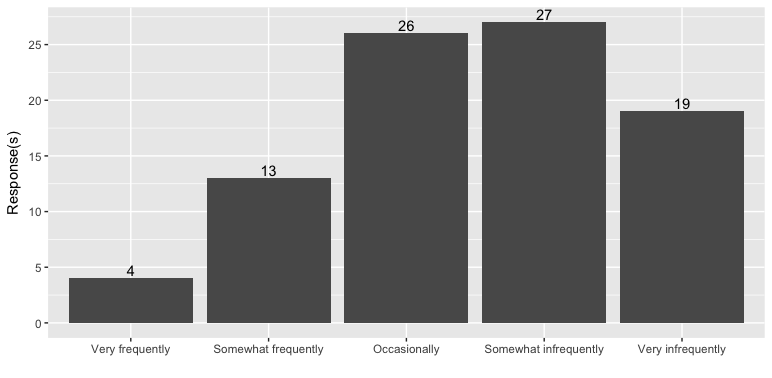
\includegraphics[width=0.95\textwidth,keepaspectratio]{FirstAttemptFailure}}
	\caption{Frequency of Failures in First Attempts at Merge Conflict Resolution. Scale: 1 is \textit{Very frequently} and 5 is \textit{very infrequently}. 89 out of 102 participants (87.26\%) indicated a frequency in the \textit{Processes Survey}~(S1).\vspace*{-0.3\baselineskip}}
	\label{fig:first-attempt-failure}
\end{figure}

Furthermore, we asked survey participants to describe their backup strategies when their first attempt at resolving a merge conflict fails.
We received 75 responses and the aggregate results are presented in Table~\ref{backup-strategies}, ranked according to the percentage of participants that described using each backup strategy.

Developers' backup strategies include \textit{take it offline} (B1), \textit{collaborating} (B2), \textit{try again} (B3), \textit{redoing changes} (B4), and \textit{no backup strategy} (B5).
Since \textit{no backup strategy} (B5) is not a strategy in and of itself, we focus on strategies B1--B4 instead.

The \textit{take it offline} (B1) strategy involves moving conflicting code away from shared branches or code repositories, and working locally to resolve the conflict without disrupting other developers.
The antithesis of this strategy is \textit{collaborating} (S2), where developers seek out other developers that are more knowledgeable about the area of conflicting code.
The B1 and B2 strategies contrast each other, and show that developers reserve more costly strategies (in terms of time, effort, and coordination) as backups to their primary resolution strategies.
The most common backup strategies, are in a way, opposite of the primary strategies.

Additionally, we find that developers also simply \textit{try again} (B3) to merge the same code together and hope that their tools are able to succeed with a second attempt.
Developers also resort to \textit{redoing changes} (B4), by way of reverting and manually recreating the changes found in conflicting commits when their initial attempt failed.
The B3 and B4 strategies appear to cement the extremes of the cost spectrum of backup strategies for resolving merge conflicts.
Simply retrying the same merge (B3) requires very little additional work.
It implies that developers think that they might have missed something, and that by going through the changes again, they might catch or have a better understanding of the two changes that are conflicting.
However, the process of redoing changes (B4) is a duplication of previous efforts. %and is therefore costly on developer's time.
This \textit{Nuclear Option} is clearly a time-consuming strategy for developers (both in planning and implementing a resolution), and yet the perceived costs of trying to unravel the conflicting code appear to be higher than the costs of reimplementing features.

\begin{table}[!htbp]
\renewcommand{\arraystretch}{1.2}
\caption{Backup Strategies for Resolving Merge Conflicts from Processes Survey (S1)}
\label{backup-strategies}
\centering
\begin{tabularx}{\textwidth}{c|l|c|r}
\toprule
  \parnoteclear % tabularx will otherwise add each note thrice
  Strategy & Description & \# Participants\parnote{75 out of 102 participants (73.53\%) provided a description of their backup strategy.\vspace*{-0.3\baselineskip}} & Percentage (\%)\textsuperscript{i} \\
\midrule
  B1 & Take it offline & 19 & 25.33\% \\
  B2 & Collaborating & 17 & 22.67\% \\
  B3 & Try again & 15 & 20.00\% \\
  B4 & Redoing changes & 14 & 18.67\% \\
  B5 & No backup strategy\hspace{2.0cm} & 10 & 13.33\% \\
\bottomrule
\end{tabularx}
\parnotes
\end{table}
\vspace{0.8em}

\boldif{Some developers do not have an approach for dealing with merge conflicts.}
Finally, an interesting result is that some developers do not have a strategy for approaching a merge conflict resolution.
The existence of this \textit{no strategy} approach is anecdotal, but curious, since we assume that developers are rational actors seeking to organize themselves in ways that increase the likelihood of successful outcomes.
Yet this strategy appears to go counter to that notion.
One explanation for the lack of a strategy is the lack of experience.
With a mean of 3.5 years of programming experience (5.6 years less than the overall mean), these participants might not have encountered enough situations to form a coherent strategy.

Interestingly, when developers perceive a merge conflict to be too difficult to resolve they occasionally resort to removing all conflicting code and reimplementing the underlying functionality in order to fix it.

%!TEX root = main.tex

\subsection{\textbf{RQ2:} What difficulties do software developers experience when managing merge conflicts?}\label{RQ2}

To understand the difficulties for software developers when encountering a merge conflict, we asked interview participants to reflect on situations when they initially face a merge conflict: what kind of information do they seek, how do they approach the resolution of the conflict, and what tools do they use. 

\subsubsection{Difficulty Factors}\label{difficulty-factors}

From the card sorting of the interview answers (Section~\ref{interviews}), we identified nine factors that developers consider when approaching a conflict and attempting to determine its difficulty (see Table~\ref{s2_factors}). 
We asked \textit{Barrier Survey}~(S2) participants to rate how each of these nine factors affected their perceptions of difficulty when approaching a merge conflict.

We received 162 responses and present the aggregated results in Table~\ref{s2_factors}; ranked according to the mean score for each factor.
Here, we discuss in detail the top 4 factors with a mean score greater than $3.00$.
These factors can be grouped into themes of \textit{technical aspects} and \textit{expertise,} and our results are presented according to these groups.

\begin{table}[!htbp]
\renewcommand{\arraystretch}{1.2}
\caption{Difficulty Factors of Merge Conflicts from Barriers Survey (S2)}
\label{s2_factors}
\centering
\begin{tabularx}{\textwidth}{>{\rowmac}c | >{\rowmac}l | *1{>{\rowmac}c} | *2{>{\rowmac}c}<{\clearrow}}
\toprule
  \parnoteclear % tabularx will otherwise add each note thrice
  Factor & Description & \likertscale{1,2,3,4,5} & Median\parnote{Responses on 5-point Likert scale indicating the degree of effect on resolution difficulty (1 indicates \textit{no effect}, 5 indicates \textit{great effect}).} & Mean\textsuperscript{i} \\
\midrule
  \setrow{\bfseries}F1 & Complexity of conflicting lines of code & \likertplot{coordinates {(1,5)(2,29)(3,38)(4,56)(5,34)}}{28.2}{5,29,38,56,34} & 4 & 3.52 \\
  \setrow{\bfseries}F2 & Expertise in area of conflicting code & \likertplot{coordinates {(1,5)(2,23)(3,50)(4,54)(5,30)}}{28.2}{5,23,50,54,30} & 4 & 3.50 \\
  \setrow{\bfseries}F3 & Complexity of files with conflicts & \likertplot{coordinates {(1,8)(2,34)(3,49)(4,51)(5,18)}}{28.2}{8,34,49,51,18} & 3 & 3.23 \\
  \setrow{\bfseries}F4 & Number of conflicting lines of code & \likertplot{coordinates {(1,2)(2,40)(3,64)(4,45)(5,11)}}{28.2}{2,40,64,45,11} & 3 & 3.14 \\
  F5 & Time to resolve a conflict & \likertplot{coordinates {(1,14)(2,56)(3,51)(4,25)(5,15)}}{28.2}{14,56,51,25,15} & 3 & 2.82 \\
  F6 & Atomicity of changesets in conflict & \likertplot{coordinates {(1,20)(2,48)(3,51)(4,29)(5,13)}}{28.2}{20,48,51,29,13} & 3 & 2.80 \\
  F7 & Dependencies of conflicting code & \likertplot{coordinates {(1,20)(2,56)(3,39)(4,33)(5,14)}}{28.2}{20,56,39,33,14} & 3 & 2.78 \\
  F8 & Number of files in the conflict & \likertplot{coordinates {(1,10)(2,69)(3,50)(4,26)(5,6)}}{28.2}{10,69,50,26,6} & 3 & 2.68 \\
  F9 & Non-functional changes in codebase & \likertplot{coordinates {(1,47)(2,63)(3,31)(4,15)(5,4)}}{28.2}{47,63,31,15,4} & 2 & 2.16 \\
\bottomrule
\end{tabularx}
\parnotes
\end{table}

\nsubsection{Technical Aspects}\label{artifact-based-factors}
Two of the top four factors refer to the perceptions about the complexity of merge conflicts (F1, F3), with the third factor being \textit{number of conflicting lines of code} (F4), which can be construed as a specific metric for the complexity of the conflict. 
While developers mentioned complexity of the lines of code and the file, none mentioned using any metrics, such as cyclomatic complexity~\cite{fenton2000quantitative,mccabe1976complexity}, Function Point Analysis~\cite{garmus2001fpa,symons1988function} etc. 
Instead, developers made educated guesses on the complexity of the code based on their own experience of either writing the code, or having worked with it. 
Some of the simple to compute metrics, such as \textit{number of conflicting lines of code} (F4), \textit{number of files in the conflict} (F8), \textit{atomicity of changesets in conflict} (F6), and the \textit{time to resolve a conflict} (F5) were mentioned. 
The only factor where static analysis tools can help was in identifying the \textit{dependencies of conflicting code} (F7).
This indicates that understanding the complexity of the conflicting code is important, but developers do not use the metrics that have been proposed by research.
While some of the simple proxies for complexity are used, developers primarily rely on their own judgement of the complexity of a conflict.

This perception of the conflict complexity can affect whether a developer resolves the conflict immediately (when small), or whether they should wait to examine the conflict when further resources are available; P8 commented:
\begin{quoting}
\textit{``Small is always easy. A 1-line merge conflict is always easier to resolve than a 400-line merge conflict, and can be done now.''}
\end{quoting}

If a merge conflict is perceived to be large or complex, a developer may decide to forgo attempting to resolve it through code manipulation and choose to revert the changes instead~\cite{Guzzi2015}.
This ``nuclear option'' requires developers to disrupt the development flow, set aside their current development work, and potentially remove good, working code that was not part of the conflict in order to return to a non-conflicting state.
In the interview, P1 describes this process as:
\begin{quoting}
\textit{``If you have many conflicts involved, many commits in the conflict...throw one of the branches away. You cannot combine tens of commits conflicting...it's not sane!''}
\end{quoting}

Further, when integrators are preparing code for production environments they prioritize merge conflicts for code review based upon the perceived difficulty of resolving the affected code.
We find that these decisions rely on human judgement factors as much as they rely on data-driven metrics.
Developers may not have the time to compute project-wide complexity metrics, such as those proposed in  literature.
Therefore, we need metrics that can be easily calculated by unexperienced developers as they face a conflict. 
%are human-aware and take into account the perceived difficulties of merge conflicts.

\nsubsection{Expertise}\label{knowledge-based-factors}
Our findings show that \textit{expertise in the area of conflicting code}~(F2) is one of the top factors in determining the difficulty of a merge conflict. 
This reiterates the fact that developers rely on their own knowledge about the conflicting codebase when approaching a conflict. 
And as seen in Section~\ref{RQ1c}, this expertise has a direct impact on the ability of developers to use \textit{code looks correct (i.e. visual test passes)} (C3) as a strategy for evaluating merge conflict resolutions.

Our results indicate that when developers feel they don't have the expertise in the conflicting codebase, they consider the conflict difficult to merge and seek out more information or assistance from others.
P5 illustrated this need for expertise when describing his workflow: 
\begin{quoting}
	\textit{``A lot of what I work on is in my own little area \textellipsis I know what to do [\textellipsis]. But in [unfamiliar part of code,] then I'll get someone else to resolve the merge conflict for me. It's someone else's code, and I don't want to screw it up.''}
\end{quoting}

Our findings confirm the need for tools that identify appropriate experts~\cite{CostaSarma} and encourage further research into selection of knowledgeable developers for merge conflict resolution.

%%%%%%%%%%%%%%%%%%%%%%%%%%%%%%%%%%%%%%%%%%%%%%%%%%%%%%%%%%%%%%%%%

%\subsubsection{Interviews}
%%The interview results suggest that developers approach merge conflicts...
%
%\subsubsection{Survey}
%Our survey suggests that regardless of gender, developer role, experience level, project size, and source distribution model, software practitioners say that the following factors affect the difficulty of a merge conflict most: 
%\begin{itemize}
%\item \textit{Complexity of conflicting lines of code}
%\item \textit{Your knowledge/expertise in area of conflicting code}
%\end{itemize}
%
%Similarly, software practitioners across every measured demographic perceived the following factors to be less important when deciding the difficulty of a merge conflict:
%\begin{itemize}
%\item \textit{Non-functional changes (whitespace, renaming, etc)}
%\item \textit{Number of files in the conflict}
%\end{itemize}
%
%While survey participants did not agree that non-functional changes strongly factor into the difficulty of a merge conflict, it is still worth noting that several interview participants named non-functional changes, such as large refactor or reformatting changes, as a cause for merge conflicts. This suggests that non-functional changes may increase the likelihood of a merge conflict happening, but they do not contribute to the conflict's difficulty.
%
%However, some demographics do view certain difficulties. For instance, open-source developers think that \textit{Atomicity of change sets in the conflict} impacts the difficulty, while closed-source developers and people who split their time evenly think that atomic change sets have no effect on the difficulty. This may be explained by the findings in Rigby et al\cite{OSS_smaller_commits}, which shows that open-source projects tend to review smaller changes than closed-source projects because "The small size lets reviewers focus on the entire change, and the incrementality reduces reviewers’ preparation time and lets them maintain an overall picture of how the change fits into the system." It is possible that our result reflects this difference of culture.
%
%We also found that Project Maintainers say that \textit{Time to resolve a conflict} has an effect, while no other role agrees. This suggests that those in a maintainer role may be more subject to time-related constraints such as maintenance or release schedules. 
%
%\comment{Project Managers say no effect because they focus on project schedules, not conflict resolutions, i.e. they are higher level/abstraction?}
%
%\todo{might be previous work}
%Support and infrastructure roles (System Engineer, Sys Admin, System Architect, DevOps) emphasized that \textit{Dependencies of conflicting code on other components} have more of an effect than other roles did. This might be due to infrastructure systems being maintained in a live environment, or systems that are currently in production use and at risk of real-time dependency failures. 
%
%Developers on projects of size 1 say that \textit{Dependencies of conflicting code on other components}. Because no other project sizes agree with this idea, we hypothesize that this could be due to their high dependence on external code because of the software production limitations of a 1-developer team.
%
%We also found that the group of developers with 21-25 years of experience frequently contradicted general consensus, but it seems more likely that these differences were simply due to the group's small sample size (4).

%We asked participants how much they trust their merging, history exploration, and/or conflict resolution tools, and 57.9\% of participants reported that they trusted these tools either \textit{A Lot} or \textit{Completely}. While this is a majority of developers, this still leaves a significant number of people (42.1\%) who trust their tools \textit{A moderate amount} or \textit{A little}. Though we had the option for \textit{Not at all}, no participants selected this option, presumably because users stop using tools that they do not trust at all. While we found no previous work discussing the threshold for how much users must trust tools for a good tool experience, we postulate that users who cannot trust their tools \textit{A Lot} or \textit{Completely} will avoid relying on such tools too much.

%\subsubsection{\textbf{Old RQ3:} What unmet needs impact the difficulty of merge conflict resolutions?}

\subsubsection{Unmet Needs for Merge Conflict Resolutions}

There can often be gaps in how developers perceive the difficulty of merge conflicts and the actual hurdles that they face when resolving these conflicts. 
These gaps can then in turn affect how effective developers are at resolving the conflict.

We, therefore, asked our interview participants open-ended questions about their experiences in resolving the most recent conflicts, especially their recollection of what made the resolution difficult.
Their responses indicated that there are several unmet needs.
We identified ten needs (see Table~\ref{s2_needs}), which range from needs about the ability to understand the code, their expertise, and existing tool support.  

\begin{table}[!htbp]
\renewcommand{\arraystretch}{1.2}
\caption{Developer Needs for Merge Conflict Resolutions from Barriers Survey (S2)}
\label{s2_needs}
\centering
\begin{tabularx}{\textwidth}{>{\rowmac}c | >{\rowmac}l | *1{>{\rowmac}c} | *2{>{\rowmac}c}<{\clearrow}}
\toprule
  \parnoteclear % tabularx will otherwise add each note thrice
  Need & Description & \likertscale{1,2,3,4,5} & Median\parnote{Responses on 5-point Likert scale indicating the degree of importance to merge resolutions (1 indicates \textit{no importance}, 5 indicates \textit{great importance}).} & Mean\textsuperscript{i} \\
\midrule
  \setrow{\bfseries}N1 & Ease of understanding conflicting code & \likertplot{coordinates {(1,0)(2,14)(3,25)(4,65)(5,37)}}{28.2}{0,14,25,65,37} & 4 & 3.89 \\
  \setrow{\bfseries}N2 & Expertise in area of conflicting code & \likertplot{coordinates {(1,1)(2,17)(3,38)(4,49)(5,36)}}{28.2}{1,17,38,49,36} & 4 & 3.72 \\
  \setrow{\bfseries}N3 & Amount of info about conflicting code & \likertplot{coordinates {(1,2)(2,21)(3,38)(4,48)(5,32)}}{28.2}{2,21,38,48,32} & 4 & 3.62 \\
  \setrow{\bfseries}N4 & Tools presenting understandable info & \likertplot{coordinates {(1,4)(2,24)(3,47)(4,32)(5,34)}}{28.2}{4,24,47,32,34} & 3 & 3.48 \\
  N5 & Changing assumptions within code & \likertplot{coordinates {(1,8)(2,27)(3,45)(4,36)(5,25)}}{28.2}{8,27,45,36,25} & 3 & 3.30 \\
  N6 & Complexity of project structure & \likertplot{coordinates {(1,6)(2,38)(3,39)(4,41)(5,17)}}{28.2}{6,38,39,41,17} & 3 & 3.18 \\
  N7 & Trustworthiness of tools & \likertplot{coordinates {(1,17)(2,29)(3,39)(4,32)(5,34)}}{28.2}{17,29,39,32,34} & 3 & 3.12 \\
  N8 & Informativeness of commit messages & \likertplot{coordinates {(1,18)(2,32)(3,30)(4,44)(5,17)}}{28.2}{18,32,30,44,17} & 3 & 3.07 \\
  N9 & Project culture & \likertplot{coordinates {(1,13)(2,37)(3,43)(4,27)(5,21)}}{28.2}{13,37,43,27,21} & 3 & 3.04 \\
  N10 & Tool support for history exploration & \likertplot{coordinates {(1,16)(2,40)(3,31)(4,32)(5,22)}}{28.2}{16,40,31,32,22} & 3 & 3.03 \\
\bottomrule
\end{tabularx}
\parnotes
\end{table}

Using results from the interview, we asked S2 survey participants to rate how much each of the ten needs affected their ability to resolve the merge conflicts.
We received 141 responses using a 5-point Likert-type scale indicating the degree of effect on resolution difficulty (1 being \textit{Not at all}, 3 being \textit{A moderate amount}, and 5 being \textit{A great deal}).
Results of the survey are presented in Table~\ref{s2_needs}. 

All the unmet needs have a mean score of at least $3.03$ on the 5-point Likert-type scale, implying that all of them mattered at least a moderate amount.
We present and discuss in detail the top four unmet needs, plus additional observations regarding the other six unmet needs. 
As with the factors in the previous section, all these needs also relate to \textit{technical aspects} (e.g., understanding the conflicting code) and their \textit{expertise} in resolving conflicts.

%All of the unmet needs in Table~\ref{survey_res_diffs} can be considered important to practitioners when resolving merge conflicts, since each received a mean score of at least 3.03 on the 5-point Likert scale.
%However, practitioners primarily working on closed-source development differed in perceptions of \textit{tool support for examining development history} (N10).
%We further discuss this demographic difference in Section~\ref{oss_vs_closed_tool_support}.

\nsubsection{Technical Aspects}
Three needs among the top four relate to technical aspects of merge conflict resolution.
The \textit{understandability of conflicting code} (N1) is ranked as the most important need, with both \textit{contextual information about the conflict} (N3) and \textit{the way in which tools present relevant information} (N4) ranking in the top four.

Data from version control systems is used by developers to identify the evolution of the code~\cite{Mihai_lenses}, however, it is not easily available and requires a context switch from the code editor to the version control system~\cite{Guzzi2015}. 
Moreover, these changes are often processed in isolation, especially when there are many changes (conflicts) to process. 
Such decomposition of overall conflicting changes into smaller ``chunks" is needed to be able to manage the complexity of the resolution process; however, this occludes viewing the changes in a larger context. 
Often developers deal with the decomposed (smaller) changes, hoping that they will all together work out. 
For example, P1 compared the resolution hurdles between two conflicts, where one was simple, and the other spanned multiple files and complex blocks of code.
\begin{quoting}
\textit{``You focus on understanding the small change, not the big one. It's easier to understand... get the small change to go with the flow of the bigger change.''}
\end{quoting}

Another challenge when viewing changes in isolation, is the fact that developers may miss the impact of the changes made as part of the resolution to the rest of the code base. 
Identifying the impact of changes on the rest of the code base has been repeatedly found to be a problem in collaborative development, as found by deSouza and Redmiles~\cite{deSouza2008} and more recently by Guzzi et al.~\cite{Guzzi2015}. 
The top unmet needs in our study also revolved around the challenges that developers face in how much information they had about the conflicting code (N3), and the difficulty in finding the needed information from current tools and practices (N3, N4, N8, N10). 
This indicates that despite advances in supporting parallel development practices, the right information needed to resolve conflicts is still not easily available to developers. 

Conflict resolution can sometime lead to defects in the code base. This can arise because of several reasons. For example the rationale of the two conflicting changes might be unclear and the merge might cause unintentional problems down the line. Or the resolved changes might not follow rigorous code review and testing to which the original changes were subject to.
Therefore, even when the practitioner understands the particular conflicting code, they may still need additional meta information about the rationale of changes and idea of future feature implementation. This is especially true in situations where the code base is old, and such information not readily available. During our interview, P7 commented:
\begin{quoting}
\textit{``It's harder to merge code when you're merging in some legacy code... But if you're a young team, and everybody who wrote the code is still a part of the team, it's easier.''}
\end{quoting}

\nsubsection{Expertise}
Knowledge is a key component of developer's needs when resolving merge conflicts, but along with that general knowledge is a need for expertise in the specific areas of code involved in a conflict.
Developers recognize this need as having a sizable effect on their ability to resolve a merge conflict, and selected \textit{expertise in the area of conflicting code} (N2) as the second most important need.

Examining code artifacts, reviewing change history, and reading documentation help with understanding the code when they are present and well-maintained.
However, locating and maintaining these supporting documents is not always possible.
In fact, Forward et al.~\cite{forward2002documentation} conducted a survey of 48 software developers and found that 68\% either agreed or strongly agreed that documentation is always outdated.
When these gaps arise, developers compensate by consulting experts in the area of conflicting code instead.

This result aligns with the goals of the TIPMerge tool~\cite{CostaSarma}, which seeks to locate experts that are best suited to resolve conflicts in a particular area of code.
However, TIPMerge, as well as other recommendation tools are not being used by real-world developers, as evidenced by the lack of such tools in the list of top 10 merge resolution tools (see Table~\ref{s2_toolset}).
The reason for this lack of research tools adoption requires further investigation.

Another surprising fact was that while the informative nature of commit messages (N8) and project culture (N9) were mentioned, they were not as highly ranked. % The same is true for project culture (N9). 
We had expected them to be higher based on prior work~\cite{yamauchi2014clustering, hindle2009automatic, cortes2014automatically, hattori2008nature}. 
We found no statistical differences between commercial or open source projects, including when accounting for experience levels.
Our results indicate that team practices, including writing commit messages may have matured enough, such that these factors are no longer considered critical in our sample set. 


%\nsubsection{Open-Source vs. Closed-Source Needs}\label{oss_vs_closed_tool_support} 
%It is interesting to note that for needs N1-N8 there was no statistical difference between practitioners focused on open-source and those focused on closed-source development when it comes to their conflict resolution needs.
%We found that practitioners who focus on open-source software development consider \textit{tool support for examining development history} (N10) to be the 3rd highest unmet need (mean: 3.60).
%Whereas, practitioners who focus on closed-source software development consider it to be the least impactful unmet need (mean: 2.86).
%%A Wilcoxon Signed-Ranks test indicated that open-source practitioners' ranking of N10 were statistically higher than closed-source practitioners' rankings of N10 (W = 1192.5, $p$-value = 0.02).
%
%This was also true in our interviews, with P8 stating:
%
%\begin{quoting}
%\textit{``I'm often dealing with code other people wrote. Nobody can review every pull request. So now I have to go back and do some archaeology to find out what's going on. Code is much easier to write than read.''}
%\end{quoting}
%
%This result suggests that history exploration in open-source projects is a more difficult task due to the lack of upfront planning and large number of volunteering contributors.
%%, or that tools are better at supporting history exploration in closed-source development environments.
%!TEX root = main.tex

\subsection{\textbf{RQ3:} How well do tools support developer's needs for managing merge conflicts?}\label{RQ3}

\begin{table}[!htbp]
\renewcommand{\arraystretch}{1.2}
\caption{Desired Improvements to Merge Toolsets from Barriers Survey (S2)}
\label{s2_tool_improvements}
\centering
\begin{tabularx}{\textwidth}{>{\rowmac}c | >{\rowmac}l | *1{>{\rowmac}c} | *2{>{\rowmac}c}<{\clearrow}}
\toprule
  \parnoteclear % tabularx will otherwise add each note thrice
  Imp.\parnote{Imp. = Improvement} & Description & \likertscale{1,2,3,4,5} & Median\parnote{Responses on 5-point Likert scale indicating the degree of potential impact on merge conflict processes (1 indicates \textit{no impact}, 5 indicates \textit{great impact}).} & Mean\textsuperscript{ii} \\
\midrule
  \setrow{\bfseries}I1 & Usability & \likertplot{coordinates {(1,6)(2,17)(3,32)(4,48)(5,16)}}{28.2}{6,17,32,48,16} & 4 & 3.43 \\
  \setrow{\bfseries}I2 & Filtering of relevant information & \likertplot{coordinates {(1,8)(2,15)(3,32)(4,48)(5,16)}}{28.2}{8,15,32,48,16} & 4 & 3.41 \\
  \setrow{\bfseries}I3 & Support for exploring project history & \likertplot{coordinates {(1,7)(2,21)(3,36)(4,39)(5,16)}}{28.2}{7,21,36,39,16} & 3 & 3.30 \\
  \setrow{\bfseries}I4 & Graphical information presentation & \likertplot{coordinates {(1,13)(2,26)(3,26)(4,37)(5,16)}}{28.2}{13,26,26,37,16} & 3 & 3.14 \\
  I5 & Transparent tool functionality/operations & \likertplot{coordinates {(1,16)(2,36)(3,24)(4,40)(5,3)}}{28.2}{16,36,24,40,3} & 3 & 2.82 \\
  I6 & Terminology consistent with other tools & \likertplot{coordinates {(1,23)(2,41)(3,32)(4,15)(5,8)}}{28.2}{23,41,32,15,8} & 2 & 2.53 \\
\bottomrule
\end{tabularx}
  \parnotes
\end{table}

Development tools need to be easy to use and provide contextualized, pertinent information in a manner that is easy to understand.
To investigate how well current tools satisfy the needs of practitioners, we asked interview participants open-ended questions about how they resolve merge conflicts.
We also ask about improvements that would be most valuable to them. 

Our results indicate that practitioners use a wide range of tools, with many directly using the Git command line interface. Our interview participants mentioned six different dimensions along which they would like improvements to tool support (see Table~\ref{s2_tool_improvements}). 

We framed the survey questions to validate the improvement needs expressed in our interviews, and ranked those six needs according to mean score.
Table~\ref{s2_tool_improvements} presents the needs from the survey responses ordered by their mean scores.
We received 119 responses using a 5-point Likert-type scale to indicate the usefulness of each type of tool improvement (1 being \textit{Not Useful}, 3 being \textit{Moderately Useful}, and 5 being \textit{Essential}).

In addition, we also asked participants which tools they use during conflict resolution.
We identified 105 different tools from the 115 responses. Some mentioned generic responses such as \textit{`` text editor''}, for which we create a separate category.
%We group these generic responses together where semantically similar meanings exist. 
Table~\ref{s2_toolset} lists the top 10 most common tools used by participants to resolve merge conflicts.

In examining the list of these tools, we note that practitioners most often use basic tools (e.g. Git, Vim/vi, or a Text Editor) to handle merge conflicts instead of employing specialized tools or plugins to modern IDEs. 
In this list, there is only one IDE (Eclipse), and three diff/merge toolsets (Git Diff, KDiff3, and Meld). 
This indicates that practitioners are currently not leveraging the functionalities provided by many research prototypes (e.g., Palantir~\cite{palantir}, Crystal~\cite{Brun2011}) that are specifically designed to facilitate proactive conflict detection, since they are built as plug-ins to modern IDEs. 

We next discuss the top four improvements rated by survey respondents. These are the responses that have a mean value higher than $3.00$.

\begin{table}[!htbp]
\renewcommand{\arraystretch}{1.3}
\caption{Merge Resolution Toolsets (Top 10) from Barriers Survey (S2)}
\label{s2_toolset}
\centering
\begin{tabularx}{\textwidth}{ll|c}
\toprule
  \parnoteclear % tabularx will otherwise add each note thrice
  Tool & Description & \# Participants (\%)\parnote{
  Survey participants were allowed to provide multiple tools. Each entry represents the number (and percentage) of participants that responded with that particular tool. 115 out of 162 respondents (71\%) indicated the use of at least one merge resolution tool.}\\
\midrule
  Git & Version Control System & 37 (15.68\%)\\
  Vim/vi & Text Editor & 17 (7.20\%)\\
  Text Editor (unspecified) & Text Editor & 14 (5.93\%)\\
  Git Diff & Diffing Tool & 11 (4.66\%)\\
  GitHub & Website & 11 (4.66\%)\\
  Eclipse & IDE & 10 (4.24\%)\\
  KDiff3 & Diff \& Merge & 9 (3.81\%)\\
  Meld & Diff \& Merge & 8 (3.39\%)\\
  SourceTree & Git/Hg Desktop Client & 8 (3.39\%)\\
  Sublime Text & Text Editor\hspace{3.2cm} & 7 (2.97\%)\\
\bottomrule
\end{tabularx}
\parnotes
\end{table}

\subsubsection{Better Usability}
%The right toolset is essential for efficiently developing solutions and resolving conflicts.
Usability is an important factor that determines whether a toolset supports or hinders the practitioner's workflow.
Our survey results indicate that \textit{better usability} (I1) is the most desired improvement of toolsets used for conflict resolution. 
%Based on the results of the survey, we found that practitioners rate usability as the most desired improvement for their current merge tools (I1).
While usability of a particular tool is important, the usability concerns become even more pertinent when they span multiple tools that are similar and must operate in sync with each other.
Survey results indicate that participants use an average of 2.5 tools, and as many as 7 tools, to resolve merge conflicts.
%With multiple tools being used during merging and conflict resolution, toolset fragmentation is a real concern for practitioners.
For instance, in our interview P1 demonstrated how he typically resolved a merge conflict by using four different tools and said: 
\begin{quoting}
\textit{``I have to jump around between tools and copy and paste version numbers...this is why integration matters.''}
\end{quoting}

Switching across multiple tools while resolving a conflict is disruptive and comes at a cost. Psychology studies~\cite{Meiran2000}\cite{gopher2000switching} have shown that task switching reduces performance and causes mental fatigue. 
Gerald Weinberg highlighted that context switching arising from toolset fragmentation is a big problem in engineering teams~\cite{Weinberg1992}. 

%This frustration is understandable for practitioners whose workflows frequently get interrupted by tool switches. Psychology studies~\cite{Meiran2000}\cite{gopher2000switching} have found that task switching comes with costs in performance and mental fatigue, and, in 1992, Gerald Weinberg highlighted the problem of toolset fragmentation within engineering teams~\cite{Weinberg1992}. 

\subsubsection{Better Exploration of Project History}
Practitioners have been known to use historical data to understand code evolution and development processes~\cite{Mihai_lenses}.
Version control and bug tracking systems contain a huge amount of meta-information about the evolution of code and development processes.
However, it is not easy to find the right bit of information in these large systems. 
Currently, there is insufficient support for performing detailed analysis of how a code snippet evolved over time and why. 
Better ways of exploring the project history (I3) was one of the top requested improvements in our survey. 
As P1 mentioned in the interview:
\begin{quoting}
\textit{``Give me a way to explore the history. To drill down, to go back up, you know? To resurface and understand what happened.''}
\end{quoting}


Currently, when performing any complex analysis it is easier to write stand alone scripts to extract the information. 
During the interview, P1 mentioned that he has written several scripts to locate particular historical commits that relate to a current merge conflict. 
Similarly, P9 described a tool, \texttt{git-diff}, that was developed by their team to add additional difference analysis functionality across branches:
\begin{quoting}
\textit{``git-diff will just do the diff based on the SHAs... we're adding metadata... It also hooks into GitHub labels to do some more advanced heuristics.''}
\end{quoting}

While writing these scripts allows extraction of relevant data contextualized to the need, it also leads to a proliferation of multiple scripts that are written by individual practitioners and need to be maintained or integrated.
This further adds to the problem of context-switching when practitioners must switch between multiple tools, and execute multiple scripts.

We are not the first to recognize the gap in tool support provided for analyzing development history among practitioners~\cite{Mihai_lenses, sun2015informationhistory, guo2016cold-start, yan2014miningcontracts}. 
It appears that practical applications of history exploration are still beyond the reach of practitioners. 
One of the reasons for this might be the simple set of text editors, and toolsets, that our study participants seem to prefer.

\subsubsection{Better Filtering of Less-Relevant Information}\label{better_filtering}
Tools that routinely handle large or complex datasets require filtering in order to efficiently locate desired pieces of information.
For example, when there are several commits in a pull request and multiple levels of code review at the line level.
It is difficult to extract the key issue in the pull request, which can get lost in the sea of low level details. Similarly, if there are multiple commits in a pull request or branch, it is hard to extract the right information.
Therefore, tools that provide filtering can better assist practitioners in working with large amounts of metadata associated with the changes.
\textit{Better ways of filtering out less relevant information} (I2) was selected as the second most important need; P1 explained:
\begin{quoting}
\textit{``You want to extract the relevant commits. The ones that actually clash...you want to zoom in on them and understand just enough and don't waste time.''}
\end{quoting}

While improvements in history exploration (I3) will make project metadata more accessible, improvements in filtering for relevant metadata will allow practitioners to focus on the relevant parts of the code impacted by the merge conflict.

%Version control systems (VCS) and bug tracking systems provide insufficient support for detailed analysis of software evolution and information retrieval~\cite{fischer2003release_history}.
%For software practitioners using \texttt{git} and other VCS, it is often easier to write scripts that accommodate their particular information needs by augmenting the capabilities of the VCS.
%During the interviews, P1 described writing several scripts in order to locate particular historical commits that relate to a current merge conflict.
%P9 also described a tool, \texttt{git-diff}, developed as part of their efforts to add additional difference analysis functionality across branches:
%\begin{displayquote}
%\textit{``git-diff will just do the diff based on the SHAs... we're adding metadata and cherry picking, so the SHAs are always going to be changing... It also hooks into GitHub labels and uses the labels on the project to do some more advanced heuristics.''}
%\end{displayquote}
%\todo{Shane: This transition is a bit rough}
%In our survey results, we see that practitioners rank \textit{better ways of filtering out less relevant information} (I2) as the second highest improvement needed in modern merge toolsets.
%This suggests that further work is needed to bring these capabilities from single-purpose scripts into common toolsets used by all practitioners.
%
%\Subsubsection{Better Exploration of Project History}
%Codoban et al.~\cite{mihai_lenses} introduced the concept of the \textit{Archeology Lens} to describe examining old development history to retrieve lost knowledge and postulated that additional tool support was needed in this context.
%We also find that practitioners consider history exploration to be a major area of improvement for development toolsets.
%Among survey participants, \textit{better ways of exploring project history} (I3) ranked as the third most important improvement needed.
%During our interviews, P1 said: 
%
%\begin{displayquote}
%\textit{``Give me a way to explore the history. To drill down, to go back up, you know? To resurface and understand what happened.''}
%\end{displayquote}
%
%The gap in support for analyzing development history among practitioner toolsets has previously been recognized by researchers~\cite{sun2015informationhistory, guo2016cold-start, yan2014miningcontracts}, however practical application of these efforts appear to have not yet reached practitioners.

\subsubsection{Better Graphical Presentation of Information}
The usefulness of information is helped or hindered by the way in which it is presented to users.
In our survey results, we found that \textit{better graphical presentation of information} (I4) was ranked the fourth highest improvement needed (mean: 3.14).

In our interviews, several practitioners reported experiencing issues with inconsistent terminology, inconsistent visual metaphors (e.g. colors, notifications, etc.), and the organizational layout of different development tools.
The cost of context switching in software development is well-known to researchers~\cite{czerwinski2004taskswitching, li2007cost_of_context_switch, blackwell2002attentioninvestment, convertino2003dualview}, and our results indicate that switching between different terminology and information presentation styles can also be a problem.
There is a need for tools that share commonality in both terminology and presentation. 

%\begin{figure*}[!htbp]
%\centering
%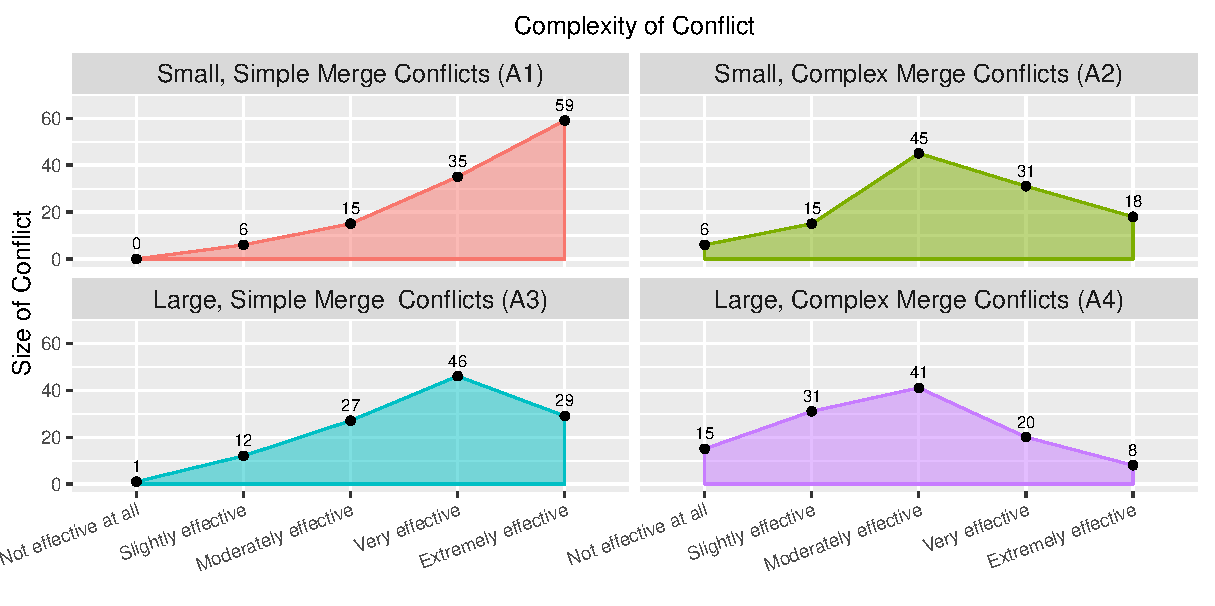
\includegraphics[width=0.92\textwidth]{ConflictComplexityVsSize.pdf}
%\caption{Effectiveness of practitioners' toolsets in supporting perceived size and complexity of merge conflicts, split on development experience. Bubble values indicate number of survey responses for effectiveness of a particular merge conflict size and complexity, and bubble size indicates the number of responses for comparison purposes.\vspace*{-0.5\baselineskip}}
%\label{size_vs_complexity}
%\end{figure*}

%\begin{table}[!htbp]
%\renewcommand{\arraystretch}{1.3}
%\caption{Practitioners' Trust in their Merging, History Exploration, and Conflict Resolution Tools\textsuperscript{i}}
%\label{survey_tool_trust}
%\centering
%\begin{tabularx}{0.65\textwidth}{@{}r|*{10}{C}c@{}}
%\toprule
%Trust Level & Response Count & Response \%\\
%\midrule
%Completely & 20 & 16.52\\
%A lot & 50 & 41.32\\
%A moderate amount & 41 & 33.88\\
%A little & 10 & 8.26\\
%Not at all & 0 & 0.00\\
%\bottomrule
%	\multicolumn{3}{c}{\noindent\parbox[t]{7.8cm}{\vspace{-3px}\textsuperscript{i}\hspace{0.2em}Survey respondents answered on a 5-point Likert-type scale indicating trust in their toolset (1 being \textit{Not at all} and 5 being \textit{Completely}).}}
%\end{tabularx}
%\end{table}

\subsubsection{Tool Mistrust/Transparency}\label{tool_trust}
Most merge tools attempt to resolve conflicts using a variety of algorithms, but revert to manual resolution when these algorithms fail.
Several interview participants indicated that they mistrust merge tools when they obscure the steps and rationale for particular results when resolving merge conflicts.
The opaque nature of history exploration tools was also found to be a source of practitioners' overall mistrust of their toolsets.
P4 commented:
\begin{quoting}
\textit{``I've never trusted the merge tools or diff tools... Sometimes I'll even manually go and do the merge myself rather than use a tool. Just because I've had several times where it's a bad merge, and I broke some code.''}
\end{quoting}

Based upon this theme of mistrust, we asked survey participants to rate the degree to which they trust their merging, history exploration, and conflict resolution tools.
We received 121 responses to this question, with a mean score of 3.66 placing the most common responses between \textit{a moderate amount} and \textit{a lot} of trust (Table~\ref{survey_tool_trust}).
Assuming that responses of \textit{a moderate amount}, \textit{a little}, or \textit{not at all} indicate some degree of mistrust, we find that 42.15\% of practitioners experience some gap in toolset trust.

However, the severity of toolset mistrust is not as significant as our interview results suggested.
Only 8.26\% of practitioners indicated that they trust their toolset \textit{a little} or \textit{not at all} (10 out of 121 responses).
As the results of the survey were counter to our interview results, we looked further. We found that: (1) participants reported on the trust levels of the tools that they regularly use, and (2) a large number of participants reported that they had discontinued toolsets when they ran into errors. This indicates that if participants had reported their trust level of these discontinued tools the results would have been lower.

\subsubsection{Perceptions of Tool Effectiveness}\label{tool_effectiveness}
The perceived size and complexity of merge conflicts affect the way in which practitioners plan, allocate, and enact resolutions.
To understand the degree to which these two factors impact practitioners' perceptions about the effectiveness of their toolsets, we asked survey participants to rate their toolset across four different merge conflict archetypes: (A1) \textit{simple, small merge conflicts}, (A2) \textit{simple, large merge conflicts}, (A3) \textit{complex, small merge conflicts}, and (A4) \textit{complex, large merge conflicts}.

Since individual participants have different toolsets, and consider different factors when determining the perceived size and complexity of a merge conflict, we instructed participants to rate their own toolset against these archetypes using their notion of what constitutes a simple vs. complex and small vs. large merge conflict.

Fig.~\ref{size_vs_complexity} provides a visual illustration of the results of this survey question.
The four plots display the results for each of the archetypes, with archetype (A1) in the top-left plot, (A2) in bottom-left plot, (A3) in the top-right plot, and (A4) in the bottom-right plot.
Individual plots are composed of a horizontal axis containing participants' software development experience, which we collect since experience can determine the range of conflicts that they have faced and their perceptions.
The vertical axis shows the range of possible responses for the effectiveness of merge toolsets.
The size and number within each bubble represent the number of respondents with a particular amount of software development experience that rated their toolset at that specific effectiveness level.

For example, a practitioner with 6-10 years of experience who indicates that her merge toolset is \textit{Extremely Effective} for \textit{small, simple merge conflicts} would be represented in the largest bubble (containing 19) in A1. % in the top-left plot. 
She would also be represented in the largest bubble (containing 13) in the bottom-right plot (A4) if she indicated that her merge toolset was \textit{Moderately effective} for \textit{large, complex merge conflicts}.

Observing the overall trends when moving between plots, we find that practitioners perceive complexity of the conflict to have a greater impact on the effectiveness of their merge toolsets than the size of merge conflicts.
Numerical analysis confirms this when finding that the mean response for archetype (A1) is 4.278 (where 5 is \textit{Extremely Effective} and 1 is \textit{Not effective at all}), (A2) is 3.782, (A3) is 3.347, and (A4) is 2.783.
The shift from \textit{small} to \textit{large} merge conflict size (A1 to A2) results in a difference in mean responses of 0.496, whereas the shift from \textit{simple} to \textit{complex} merge conflict complexity results in a difference in mean responses of 0.930.

These results suggest that merge tools are currently equipped to handle increases in the size of merge conflicts, but not as well equipped for increases in complexity.
The increasing amount of code being developed in distributed environments means that scaling support in both dimensions is necessary to accommodate practitioners' needs.
%!TEX root = main.tex

\vspace*{1.8\baselineskip}
\section{What difficulties do software developers experience when managing merge conflicts? (RQ4)}\label{RQ4}

To understand the difficulties software developers face when managing merge conflicts, we asked interview participants to reflect on situations when they faced a merge conflict.
Based on responses in the \textit{Exploratory Interviews}, we asked \textit{Barriers Survey} participants to rate the resulting factors and needs.

\subsection{Difficulty Factors}\label{difficulty-factors}

We identified nine factors that developers consider when approaching a conflict and attempting to determine its difficulty (see Table~\ref{s2_factors}).
We asked \textit{Barrier Survey} participants to rate how each of these nine factors affected their perceptions of difficulty when approaching a merge conflict.

We received 162 responses and present the aggregated results in Table~\ref{s2_factors}; ranked according to the mean score for each factor.
Here, we discuss in detail the top 4 factors with a mean score greater than $3.00$.
These factors can be grouped into \textit{technical aspects} and \textit{expertise,} and our results are presented according to these groups.

\begin{table}[!htbp]
\renewcommand{\arraystretch}{1.2}
\caption{Difficulty Factors of Merge Conflicts from \textit{Barriers Survey}}
\label{s2_factors}
\centering
\begin{tabularx}{\textwidth}{cl*1{c}A{1.03cm}A{1.03cm}}
\toprule
  \belowrulesepcolor{shaded}
  \rowcolor[gray]{0.85}
  \parnoteclear % tabularx will otherwise add each note thrice
  Factor & Description & \likertscale{1,2,3,4,5} & Median\parnote{Responses on 5-point Likert-type scale indicating the degree of effect on resolution difficulty (1 indicates \textit{no effect}, 5 indicates \textit{great effect}).} & Mean\textsuperscript{i} \\
  \aboverulesepcolor{shaded}
\midrule
  F1 & Complexity of conflicting lines of code & \likertplot{coordinates {(1,5)(2,29)(3,38)(4,56)(5,34)}}{28.2}{5,29,38,56,34} & 4 & 3.52 \\
  \rowcolor[gray]{0.95}F2 & Expertise in area of conflicting code & \likertplot{coordinates {(1,5)(2,23)(3,50)(4,54)(5,30)}}{28.2}{5,23,50,54,30} & 4 & 3.50 \\
  F3 & Complexity of files with conflicts & \likertplot{coordinates {(1,8)(2,34)(3,49)(4,51)(5,18)}}{28.2}{8,34,49,51,18} & 3 & 3.23 \\
  \rowcolor[gray]{0.95}F4 & Number of conflicting lines of code & \likertplot{coordinates {(1,2)(2,40)(3,64)(4,45)(5,11)}}{28.2}{2,40,64,45,11} & 3 & 3.14 \\
  F5 & Time to resolve a conflict & \likertplot{coordinates {(1,14)(2,56)(3,51)(4,25)(5,15)}}{28.2}{14,56,51,25,15} & 3 & 2.82 \\
  \rowcolor[gray]{0.95}F6 & Atomicity of changesets in conflict & \likertplot{coordinates {(1,20)(2,48)(3,51)(4,29)(5,13)}}{28.2}{20,48,51,29,13} & 3 & 2.80 \\
  F7 & Dependencies of conflicting code & \likertplot{coordinates {(1,20)(2,56)(3,39)(4,33)(5,14)}}{28.2}{20,56,39,33,14} & 3 & 2.78 \\
  \rowcolor[gray]{0.95}F8 & Number of files in the conflict & \likertplot{coordinates {(1,10)(2,69)(3,50)(4,26)(5,6)}}{28.2}{10,69,50,26,6} & 3 & 2.68 \\
  F9 & Non-functional changes in codebase\hspace{1.2cm} & \likertplot{coordinates {(1,47)(2,63)(3,31)(4,15)(5,4)}}{28.2}{47,63,31,15,4} & 2 & 2.16 \\
\bottomrule
\end{tabularx}
\parnotes
\end{table}\vspace{2.1em}

\subsection{Technical Aspects}\label{artifact-based-factors}
Two of the top four factors refer to the perceptions about the complexity of merge conflicts (F1, F3), with the fourth factor being \textit{number of conflicting lines of code} (F4), which can be construed as a specific metric for the complexity of the conflict. 
While developers mentioned complexity of the lines of code and the file, none mentioned using any metrics, such as cyclomatic complexity~\cite{fenton2000quantitative,mccabe1976complexity} or Function Point Analysis~\cite{garmus2001fpa,symons1988function}. 
Instead, developers made educated guesses on the complexity of the code based on their own experience of either writing the code, or having worked with it. 
Some of the simple-to-compute metrics, such as the \textit{number of conflicting lines of code} (F4), the \textit{number of files in the conflict} (F8), the \textit{atomicity of changesets in conflict} (F6), and the \textit{time to resolve a conflict} (F5) were mentioned.

Research has shown~\cite{gil_correlation_2017} that the size of the code is the most important predictive feature for external factors (e.g. bugs) of all proposed complexity measures.
This suggests that it might be enough for developers to rely on it when assessing the complexity of the conflicting code.
However, we find that the impacts of size differ from those of complexity measures when developers provide their own definitions for these measures (see Section~\ref{tool_effectiveness}).

The only factor where static analysis tools can help was in identifying the \textit{dependencies of conflicting code} (F7).
This indicates that understanding the complexity of the conflicting code is important, but developers do not use the metrics that have been proposed by research.
While some of the simple proxies for complexity are used, developers primarily rely on their own judgement of the complexity of a conflict.
This perception of the conflict complexity can affect whether a developer resolves the conflict immediately, or whether they should wait to examine the conflict when further resources are available. In the interviews, P8 commented:
\begin{quoting}
\textit{``Small is always easy. A 1-line merge conflict is always easier to resolve than a 400-line merge conflict.''}
\end{quoting}

If a merge conflict is perceived to be large or complex, a developer may decide to forgo attempting to resolve it through code manipulation and choose to revert the changes instead~\cite{Guzzi2015}.
This \emph{``nuclear option''} requires developers to disrupt the development flow, set aside their current development work, and potentially remove good, working code that was not part of the conflict in order to return to a non-conflicting state.
In the interview, P1 describes this process as:
\begin{quoting}
\textit{``If you have many conflicts involved, many commits in the conflict... throw one of the branches away. You cannot combine tens of commits conflicting... it's not sane!''}
\end{quoting}

Further, when integrators are preparing code for production environments they prioritize merge conflicts for code review based upon the perceived difficulty of resolving the affected code.
We find that these decisions rely on human judgement factors as much as they rely on data-driven metrics.
Developers may not have the time to compute project-wide complexity metrics, such as those proposed in literature.
Instead, they use educated guesses and intuition based on familiarity with the codebase; either from writing the code, or having worked with it.
Therefore, we need metrics that can be easily calculated by unexperienced developers as they face a conflict. 
%are human-aware and take into account the perceived difficulties of merge conflicts.

\subsection{Expertise}\label{knowledge-based-factors}

Our findings show that the \textit{expertise in the area of conflicting code}~(F2) is one of the top factors in determining the difficulty of a merge conflict. 
This reiterates the fact that developers rely on their own knowledge about the conflicting codebase when approaching a conflict. 
And as seen in Section~\ref{RQ3}, this expertise has a direct impact on the ability of developers to use \textit{code looks correct (i.e. visual test passes)} (C3) as a strategy for evaluating merge conflict resolutions.

Our results indicate that when developers feel they don't have the expertise in the conflicting codebase, they consider the conflict difficult to merge and seek out more information or assistance from others.
P5 illustrated this need for expertise when describing his workflow: 
\begin{quoting}
	\textit{``A lot of what I work on is in my own little area \textellipsis I know what to do [\textellipsis]. But in [an unfamiliar part of the code,] then I'll get someone else to resolve the merge conflict for me. It's someone else's code, and I don't want to screw it up.''}
\end{quoting}

Our findings confirm the need for tools that identify appropriate experts~\cite{CostaSarma} and encourage further research into selection of knowledgeable developers for merge conflict resolution.

%%%%%%%%%%%%%%%%%%%%%%%%%%%%%%%%%%%%%%%%%%%%%%%%%%%%%%%%%%%%%%%%%

%\subsubsection{Interviews}
%%The interview results suggest that developers approach merge conflicts...
%
%\subsubsection{Survey}
%Our survey suggests that regardless of gender, developer role, experience level, project size, and source distribution model, software practitioners say that the following factors affect the difficulty of a merge conflict most: 
%\begin{itemize}
%\item \textit{Complexity of conflicting lines of code}
%\item \textit{Your knowledge/expertise in area of conflicting code}
%\end{itemize}
%
%Similarly, software practitioners across every measured demographic perceived the following factors to be less important when deciding the difficulty of a merge conflict:
%\begin{itemize}
%\item \textit{Non-functional changes (whitespace, renaming, etc)}
%\item \textit{Number of files in the conflict}
%\end{itemize}
%
%While survey participants did not agree that non-functional changes strongly factor into the difficulty of a merge conflict, it is still worth noting that several interview participants named non-functional changes, such as large refactor or reformatting changes, as a cause for merge conflicts. This suggests that non-functional changes may increase the likelihood of a merge conflict happening, but they do not contribute to the conflict's difficulty.
%
%However, some demographics do view certain difficulties. For instance, open-source developers think that \textit{Atomicity of change sets in the conflict} impacts the difficulty, while closed-source developers and people who split their time evenly think that atomic change sets have no effect on the difficulty. This may be explained by the findings in Rigby et al\cite{OSS_smaller_commits}, which shows that open-source projects tend to review smaller changes than closed-source projects because "The small size lets reviewers focus on the entire change, and the incrementality reduces reviewers’ preparation time and lets them maintain an overall picture of how the change fits into the system." It is possible that our result reflects this difference of culture.
%
%We also found that Project Maintainers say that \textit{Time to resolve a conflict} has an effect, while no other role agrees. This suggests that those in a maintainer role may be more subject to time-related constraints such as maintenance or release schedules. 
%
%\comment{Project Managers say no effect because they focus on project schedules, not conflict resolutions, i.e. they are higher level/abstraction?}
%
%\todo{might be previous work}
%Support and infrastructure roles (System Engineer, Sys Admin, System Architect, DevOps) emphasized that \textit{Dependencies of conflicting code on other components} have more of an effect than other roles did. This might be due to infrastructure systems being maintained in a live environment, or systems that are currently in production use and at risk of real-time dependency failures. 
%
%Developers on projects of size 1 say that \textit{Dependencies of conflicting code on other components}. Because no other project sizes agree with this idea, we hypothesize that this could be due to their high dependence on external code because of the software production limitations of a 1-developer team.
%
%We also found that the group of developers with 21-25 years of experience frequently contradicted general consensus, but it seems more likely that these differences were simply due to the group's small sample size (4).

%We asked participants how much they trust their merging, history exploration, and/or conflict resolution tools, and 57.9\% of participants reported that they trusted these tools either \textit{A Lot} or \textit{Completely}. While this is a majority of developers, this still leaves a significant number of people (42.1\%) who trust their tools \textit{A moderate amount} or \textit{A little}. Though we had the option for \textit{Not at all}, no participants selected this option, presumably because users stop using tools that they do not trust at all. While we found no previous work discussing the threshold for how much users must trust tools for a good tool experience, we postulate that users who cannot trust their tools \textit{A Lot} or \textit{Completely} will avoid relying on such tools too much.

%\subsubsection{\textbf{Old RQ3:} What unmet needs impact the difficulty of merge conflict resolutions?}

\subsection{Unmet Needs for Merge Conflict Resolutions}

There can often be gaps in how developers perceive the difficulty of merge conflicts and the actual hurdles that they face when resolving these conflicts. 
These gaps can then in turn affect how effective developers are at resolving the conflict.

We, therefore, asked our interview participants open-ended questions about their experiences in resolving the most recent conflicts, especially their recollection of what made the conflict resolution difficult.
Their responses indicated that there are several unmet needs.
We identified ten needs (see Table~\ref{s2_needs}), which range from needs about the ability to understand the code, their expertise, and existing tool support.  

\begin{table}[!htbp]
\renewcommand{\arraystretch}{1.2}
\caption{Developer Needs for Merge Conflict Resolutions from \textit{Barriers Survey}}
\label{s2_needs}
\centering
\begin{tabularx}{\textwidth}{cl*1{c}A{1.03cm}A{1.03cm}}
\toprule
  \belowrulesepcolor{shaded}
  \rowcolor[gray]{0.85}
  \parnoteclear % tabularx will otherwise add each note thrice
  Need & Description & \likertscale{1,2,3,4,5} & Median\parnote{Responses on 5-point Likert-type scale indicating the degree of importance to merge resolutions (1 indicates \textit{no importance}, 5 indicates \textit{great importance}).\vspace*{-0.3\baselineskip}} & Mean\textsuperscript{i} \\
  \aboverulesepcolor{shaded}
\midrule
  N1 & Ease of understanding conflicting code & \likertplot{coordinates {(1,0)(2,14)(3,25)(4,65)(5,37)}}{28.2}{0,14,25,65,37} & 4 & 3.89 \\
  \rowcolor[gray]{0.95}N2 & Expertise in area of conflicting code & \likertplot{coordinates {(1,1)(2,17)(3,38)(4,49)(5,36)}}{28.2}{1,17,38,49,36} & 4 & 3.72 \\
  N3 & Amount of info about conflicting code & \likertplot{coordinates {(1,2)(2,21)(3,38)(4,48)(5,32)}}{28.2}{2,21,38,48,32} & 4 & 3.62 \\
  \rowcolor[gray]{0.95}N4 & Tools presenting understandable info & \likertplot{coordinates {(1,4)(2,24)(3,47)(4,32)(5,34)}}{28.2}{4,24,47,32,34} & 3 & 3.48 \\
  N5 & Changing assumptions within code & \likertplot{coordinates {(1,8)(2,27)(3,45)(4,36)(5,25)}}{28.2}{8,27,45,36,25} & 3 & 3.30 \\
  \rowcolor[gray]{0.95}N6 & Complexity of project structure & \likertplot{coordinates {(1,6)(2,38)(3,39)(4,41)(5,17)}}{28.2}{6,38,39,41,17} & 3 & 3.18 \\
  N7 & Trustworthiness of tools & \likertplot{coordinates {(1,17)(2,29)(3,39)(4,32)(5,34)}}{28.2}{17,29,39,32,34} & 3 & 3.12 \\
  \rowcolor[gray]{0.95}N8 & Informativeness of commit messages & \likertplot{coordinates {(1,18)(2,32)(3,30)(4,44)(5,17)}}{28.2}{18,32,30,44,17} & 3 & 3.07 \\
  N9 & Project culture & \likertplot{coordinates {(1,13)(2,37)(3,43)(4,27)(5,21)}}{28.2}{13,37,43,27,21} & 3 & 3.04 \\
  \rowcolor[gray]{0.95}N10 & Tool support for history exploration\hspace{1.3cm} & \likertplot{coordinates {(1,16)(2,40)(3,31)(4,32)(5,22)}}{28.2}{16,40,31,32,22} & 3 & 3.03 \\
\bottomrule
\end{tabularx}
\parnotes
\end{table}

Using the results from the interview, we asked \textit{Barriers Survey} participants to rate how much each of the ten needs affected their ability to resolve the merge conflicts.
We received 141 responses using a 5-point Likert-type scale indicating the the effect on resolution difficulty, with 1 being \textit{Not at all}, 3 being \textit{A moderate amount}, and 5 being \textit{A great deal.}
Results of the survey are presented in Table~\ref{s2_needs}. 

All the unmet needs have a mean score of at least $3.03$ on the 5-point Likert-type scale, implying that all of them mattered at least a moderate amount.
We present and discuss in detail the top four unmet needs, plus additional observations regarding the other six unmet needs. 
As with the factors in the previous section, all these needs also relate to \textit{technical aspects} (e.g., understanding the conflicting code) and their \textit{expertise} in resolving conflicts.\vspace{2em}

\subsection{Technical Aspects}\label{technical_aspects}
Three needs among the top four relate to technical aspects of merge conflict resolution.
The \textit{understandability of conflicting code} (N1) is ranked as the most important need, with both \textit{contextual information about the conflict} (N3) and \textit{the way in which tools present relevant information} (N4) ranking in the top four.

Data from version control systems is used by developers to identify the evolution of the code~\cite{Mihai_lenses}.
However, it is not easily available and requires a context switch from the code editor to the version control system~\cite{Guzzi2015}. 
Moreover, these changes are often processed in isolation, especially when there are many changes (conflicts) to process. 
Such decomposition of overall conflicting changes into smaller ``chunks'' is needed to be able to manage the complexity of the resolution process.
However, this occludes viewing the changes in a larger context. 
Often developers deal with the decomposed (smaller) changes, hoping that they will work well together. 
For example, P1 compared the resolution hurdles between two conflicts, where one was simple, and the other spanned multiple files and complex blocks of code.
\begin{quoting}
\textit{``You focus on understanding the small change, not the big one. It's easier to understand... get the small change to go with the flow of the bigger change.''}
\end{quoting}

Another challenge when viewing changes in isolation is the fact that developers may miss the impact of the changes made as part of the resolution to the rest of the code base. 
Identifying the impact of changes on the rest of the code base has been repeatedly found to be a problem in collaborative development~\cite{deSouza2008, Guzzi2015}. 
%as found by deSouza and Redmiles~\cite{deSouza2008} and more recently by Guzzi et al.~\cite{Guzzi2015}. 
The top unmet needs in our study also revolved around the challenges that developers face in how much information they had about the conflicting code (N3), and the difficulty in finding the needed information from current tools and practices (N3, N4, N8, N10). 
This indicates that despite advances in supporting parallel development practices, the right information needed to resolve conflicts is still not easily available to developers. 

Conflict resolution can sometimes lead to defects in the code base. 
This can arise for several reasons. 
For example the rationale of the two conflicting changes might be unclear and the merge might cause unintentional problems down the line. 
Or the resolved changes might not follow rigorous code review and testing to which the original changes were subjected.
Therefore, even when the developer understands the particular conflicting code, they may still need additional meta-information about the rationale of changes and idea of future feature implementation. 
This is especially true in situations where the code base is old, and such information not readily available. During our interview, P7 commented:
\begin{quoting}
\textit{``It's harder to merge code when you're merging in some legacy code... But if you're a young team, and everybody who wrote the code is still a part of the team, it's easier.''}
\end{quoting}

\subsection{Expertise}
Knowledge is a key component of developers' needs when resolving merge conflicts.
Along with general knowledge there is a need for expertise in the specific areas of code involved in a conflict.
Developers recognize this need as having a sizable effect on their ability to resolve a merge conflict, and selected \textit{expertise in the area of conflicting code} (N2) as the second most important need.

Examining code artifacts, reviewing change history, and reading documentation helps with understanding the code when they are present and well-maintained.
However, locating and maintaining these supporting documents is not always possible.
In fact, \citet{forward2002documentation}, in a survey of 48 software developers, found that 68\% either agreed or strongly agreed that documentation is always outdated.
When these gaps arise, developers compensate by consulting experts in the area of conflicting code instead.

This result aligns with the goals of the TIPMerge tool~\cite{CostaSarma}, which seeks to locate experts that are best suited to resolve conflicts in a particular area of code.
However, TIPMerge, as well as other recommendation tools are not being used by real-world developers, as evidenced by the lack of such tools in the list of top 10 merge awareness tools (Table~\ref{s1_toolset}) and merge resolution tools (Table~\ref{s2_toolset}).
The reason for this lack of research tools adoption requires further investigation.

Another surprising fact was that while the informative nature of commit messages (N8) and project culture (N9) were mentioned, they were not as highly ranked. % The same is true for project culture (N9). 
We had expected them to be higher based on prior work~\cite{yamauchi2014clustering, hindle2009automatic, cortes2014automatically, hattori2008nature}. 
We found no statistical differences between commercial or open source projects, including when accounting for experience levels.
Our results indicate that team practices, including writing commit messages may have matured enough, such that these factors are no longer considered critical in our sample set. 


%\nsubsection{Open-Source vs. Closed-Source Needs}\label{oss_vs_closed_tool_support} 
%It is interesting to note that for needs N1-N8 there was no statistical difference between practitioners focused on open-source and those focused on closed-source development when it comes to their conflict resolution needs.
%We found that practitioners who focus on open-source software development consider \textit{tool support for examining development history} (N10) to be the 3rd highest unmet need (mean: 3.60).
%Whereas, practitioners who focus on closed-source software development consider it to be the least impactful unmet need (mean: 2.86).
%%A Wilcoxon Signed-Ranks test indicated that open-source practitioners' ranking of N10 were statistically higher than closed-source practitioners' rankings of N10 (W = 1192.5, $p$-value = 0.02).
%
%This was also true in our interviews, with P8 stating:
%
%\begin{quoting}
%\textit{``I'm often dealing with code other people wrote. Nobody can review every pull request. So now I have to go back and do some archaeology to find out what's going on. Code is much easier to write than read.''}
%\end{quoting}
%
%This result suggests that history exploration in open-source projects is a more difficult task due to the lack of upfront planning and large number of volunteering contributors.
%%, or that tools are better at supporting history exploration in closed-source development environments.
%!TEX root = main.tex

\section{How well do tools support developer's needs for managing merge conflicts? (RQ5)}\label{RQ5}

Development tools need to be easy to use and provide contextualized, pertinent information in a manner that is easy to understand.
To investigate how well current tools satisfy the needs of developers, we asked interview participants open-ended questions about how they resolve merge conflicts.
We also ask about improvements that would be most valuable to them.

We framed the \textit{Barriers Survey} questions to validate the improvement needs expressed in our interviews, and ranked those six needs according to mean score.
Table~\ref{s2_tool_improvements} presents the needs from the survey responses ordered by their mean scores.
We received 119 responses using a 5-point Likert-type scale to indicate the usefulness of each type of tool improvement (1 being \textit{Not Useful}, 3 being \textit{Moderately Useful}, and 5 being \textit{Essential}).

\begin{table}[!htbp]
\renewcommand{\arraystretch}{1.2}
\caption{Desired Improvements to Merge Toolsets from \textit{Barriers Survey}}
\label{s2_tool_improvements}
\centering
\begin{tabularx}{\textwidth}{c|Q{7.5cm}|*1{c}|A{1cm}A{1cm}}
\toprule
  \rowcolor[gray]{0.85}
  \parnoteclear % tabularx will otherwise add each note thrice
  Imp.\parnote{Imp. = Improvement} & Description & \likertscale{1,2,3,4,5} & Median\parnote{Responses on 5-point Likert-type scale indicating the degree of potential impact on merge conflict processes (1 indicates \textit{no impact}, 5 indicates \textit{great impact}).\vspace*{-0.3\baselineskip}} & Mean\textsuperscript{ii} \\
\midrule
  I1 & Usability & \likertplot{coordinates {(1,6)(2,17)(3,32)(4,48)(5,16)}}{28.2}{6,17,32,48,16} & 4 & 3.43 \\
  \rowcolor[gray]{0.95}I2 & Filtering of relevant information & \likertplot{coordinates {(1,8)(2,15)(3,32)(4,48)(5,16)}}{28.2}{8,15,32,48,16} & 4 & 3.41 \\
  I3 & Support for exploring project history & \likertplot{coordinates {(1,7)(2,21)(3,36)(4,39)(5,16)}}{28.2}{7,21,36,39,16} & 3 & 3.30 \\
  \rowcolor[gray]{0.95}I4 & Graphical information presentation & \likertplot{coordinates {(1,13)(2,26)(3,26)(4,37)(5,16)}}{28.2}{13,26,26,37,16} & 3 & 3.14 \\
  I5 & Transparent tool functionality/operations & \likertplot{coordinates {(1,16)(2,36)(3,24)(4,40)(5,3)}}{28.2}{16,36,24,40,3} & 3 & 2.82 \\
  \rowcolor[gray]{0.95}I6 & Terminology consistent with other tools\hspace{0.5cm} & \likertplot{coordinates {(1,23)(2,41)(3,32)(4,15)(5,8)}}{28.2}{23,41,32,15,8} & 2 & 2.53 \\
\bottomrule
\end{tabularx}
  \parnotes
\end{table}

Our results indicate that developers use a wide range of tools, with many directly using the Git command line interface. 
Our interview participants mentioned six different dimensions along which they would like improvements to tool support.

In addition, we also asked \textit{Barriers Survey} participants which tools they use during conflict resolution.
We identified 105 different tools from the 115 responses. 
Some mentioned generic responses such as \textit{``text editor,''} for which we create a separate category.
%We group these generic responses together where semantically similar meanings exist. 
Table~\ref{s2_toolset} lists the top 10 most common tools used by participants to resolve merge conflicts.

\begin{table}[!htbp]
\renewcommand{\arraystretch}{1.3}
\caption{Merge Resolution Toolsets (Top 10) from \textit{Barriers Survey}}
\label{s2_toolset}
\centering
\begin{tabularx}{\textwidth}{Q{4.65cm}Q{4.5cm}|cr}
\toprule
  \rowcolor[gray]{0.85}
  \parnoteclear % tabularx will otherwise add each note thrice
  Tool & Description & Participants\parnote{\label{mergetools}Survey participants were allowed to provide multiple tools. Each entry represents the number (and percentage) of participants that responded with that particular tool. 115 out of 162 participants (70.99\%) indicated the use of at least one merge resolution tool.} & Percentage\parnoteref{mergetools}\\
\midrule
  Git & Version Control System & 37 & (15.68\%)\\
  \rowcolor[gray]{0.95}Vim/vi & Text Editor & 17 & (7.20\%)\\
  Text Editor (unspecified) & Text Editor & 14 & (5.93\%)\\
  \rowcolor[gray]{0.95}Git Diff & Diffing Tool & 11 & (4.66\%)\\
  GitHub & Website & 11 & (4.66\%)\\
  \rowcolor[gray]{0.95}Eclipse & IDE & 10 & (4.24\%)\\
  KDiff3 & Diff \& Merge & 9 & (3.81\%)\\
  \rowcolor[gray]{0.95}Meld & Diff \& Merge & 8 & (3.39\%)\\
  SourceTree & Git/Hg Desktop Client & 8 & (3.39\%)\\
  \rowcolor[gray]{0.95}Sublime Text & Text Editor\hspace{3.2cm} & 7 & (2.97\%)\\
\bottomrule
\end{tabularx}
\parnotes
\end{table}

In examining the list of these tools, we note that developers most often use basic tools (e.g. Git, Vim/vi, or a Text Editor) to handle merge conflicts instead of employing specialized tools or plugins to modern IDEs. 
In this list, there is only one IDE (Eclipse), and three diff/merge toolsets (Git Diff, KDiff3, and Meld). 
Along with the list of toolsets used for evaluating whether a merge resolution was successful (see Table~\ref{resolution-evaluation-tools}), we find that developers lack proactive conflict detection tools and code analysis tools that could address many of the developer needs (see Table~\ref{s2_needs}) and desired improvements (see Table~\ref{s2_tool_improvements}).

We next discuss the top four improvements rated by survey participants. These are the responses that have a mean value higher than $3.00$.

\subsection{Better Usability}
%The right toolset is essential for efficiently developing solutions and resolving conflicts.
Usability is an important factor that determines whether a toolset supports or hinders the developer's workflow.
Our \textit{Barriers Survey} results indicate that \textit{better usability} (I1) is the most desired improvement of toolsets used for conflict resolution. 
%Based on the results of the survey, we found that practitioners rate usability as the most desired improvement for their current merge tools (I1).
While usability of a particular tool is important, the usability concerns become even more pertinent when they span multiple tools that are similar and must operate in sync with each other.
Survey results indicate that participants use an average of 2.5 tools, and as many as 7 tools, to resolve merge conflicts.
%With multiple tools being used during merging and conflict resolution, toolset fragmentation is a real concern for practitioners.
For instance, in our interview, P1 demonstrated how he typically resolved a merge conflict by using four different tools and said: 
\begin{quoting}
\textit{``I have to jump around between tools and copy and paste version numbers...this is why integration matters.''}
\end{quoting}

Switching across multiple tools while resolving a conflict is disruptive and comes at a cost. 
Psychology studies~\cite{Meiran2000,gopher2000switching} have shown that task switching reduces performance and causes mental fatigue. 
Gerald Weinberg highlighted that context switching arising from toolset fragmentation is a big problem in engineering teams~\cite{Weinberg1992}. 

%This frustration is understandable for practitioners whose workflows frequently get interrupted by tool switches. Psychology studies~\cite{Meiran2000}\cite{gopher2000switching} have found that task switching comes with costs in performance and mental fatigue, and, in 1992, Gerald Weinberg highlighted the problem of toolset fragmentation within engineering teams~\cite{Weinberg1992}. 

\subsection{Better Exploration of Project History}
Developers have been known to use historical data to understand code evolution and development processes~\cite{Mihai_lenses}.
Version control and bug tracking systems contain a huge amount of meta-information about the evolution of code and development processes.
However, it is not easy to find the right bit of information in these large systems. 
Currently, there is insufficient support for performing detailed analysis of how a code snippet evolved over time and why. 
Better ways of exploring the project history (I3) was one of the top requested improvements in our survey. 
As P1 mentioned in the interview:
\begin{quoting}
\textit{``Give me a way to explore the history. To drill down, to go back up, you know? To resurface and understand what happened.''}
\end{quoting}


Currently, when performing any complex analysis it is easier to write stand alone scripts to extract the information. 
During the interview, P1 mentioned that he has written several scripts to locate particular historical commits that relate to a current merge conflict. 
Similarly, P9 described a tool, \texttt{git-diff}, that was developed by their team to add additional difference analysis functionality across branches:
\begin{quoting}
\textit{``git-diff will just do the diff based on the SHAs... we're adding metadata... It also hooks into GitHub labels to do some more advanced heuristics.''}
\end{quoting}

While writing these scripts allows extraction of relevant data contextualized to the need, it also leads to a proliferation of multiple scripts that are written by individual developers and need to be maintained or integrated.
This further adds to the problem of context-switching when developers must switch between multiple tools, and execute multiple scripts.

We are not the first to recognize the gap in tool support provided for analyzing development history among developers~\cite{Mihai_lenses, sun2015informationhistory, guo2016cold-start, yan2014miningcontracts}. 
It appears that practical applications of history exploration are still beyond the reach of developers. 
One of the reasons for this might be the simple set of text editors, and toolsets, that our study participants seem to prefer.

\subsection{Better Filtering of Less-Relevant Information}\label{better_filtering}
Tools that routinely handle large or complex datasets require filtering in order to efficiently locate desired pieces of information.
For example, when there are several commits in a pull request and multiple code reviews documented across the new code.
It is difficult to extract the key issue in the pull request, which can get lost in the sea of low level details.
Similarly, if there are multiple commits in a pull request or branch, it is hard to extract the right information.
Therefore, tools that provide filtering can better assist developers in working with large amounts of metadata associated with the changes.
\textit{Better ways of filtering out less relevant information} (I2) was selected as the second most important need; P1 explained:
\begin{quoting}
\textit{``You want to extract the relevant commits. The ones that actually clash...you want to zoom in on them and understand just enough and don't waste time.''}
\end{quoting}

While improvements in history exploration (I3) will make project metadata more accessible, improvements in filtering for relevant metadata will allow developers to focus on the relevant parts of the code impacted by the merge conflict.

%Version control systems (VCS) and bug tracking systems provide insufficient support for detailed analysis of software evolution and information retrieval~\cite{fischer2003release_history}.
%For software practitioners using \texttt{git} and other VCS, it is often easier to write scripts that accommodate their particular information needs by augmenting the capabilities of the VCS.
%During the interviews, P1 described writing several scripts in order to locate particular historical commits that relate to a current merge conflict.
%P9 also described a tool, \texttt{git-diff}, developed as part of their efforts to add additional difference analysis functionality across branches:
%\begin{displayquote}
%\textit{``git-diff will just do the diff based on the SHAs... we're adding metadata and cherry picking, so the SHAs are always going to be changing... It also hooks into GitHub labels and uses the labels on the project to do some more advanced heuristics.''}
%\end{displayquote}
%\todo{Shane: This transition is a bit rough}
%In our survey results, we see that practitioners rank \textit{better ways of filtering out less relevant information} (I2) as the second highest improvement needed in modern merge toolsets.
%This suggests that further work is needed to bring these capabilities from single-purpose scripts into common toolsets used by all practitioners.
%
%\Subsubsection{Better Exploration of Project History}
%Codoban et al.~\cite{mihai_lenses} introduced the concept of the \textit{Archeology Lens} to describe examining old development history to retrieve lost knowledge and postulated that additional tool support was needed in this context.
%We also find that practitioners consider history exploration to be a major area of improvement for development toolsets.
%Among survey participants, \textit{better ways of exploring project history} (I3) ranked as the third most important improvement needed.
%During our interviews, P1 said: 
%
%\begin{displayquote}
%\textit{``Give me a way to explore the history. To drill down, to go back up, you know? To resurface and understand what happened.''}
%\end{displayquote}
%
%The gap in support for analyzing development history among practitioner toolsets has previously been recognized by researchers~\cite{sun2015informationhistory, guo2016cold-start, yan2014miningcontracts}, however practical application of these efforts appear to have not yet reached practitioners.

\subsection{Better Graphical Presentation of Information}
The usefulness of information is helped or hindered by the way in which it is presented to users.
In our survey results, we found that \textit{better graphical presentation of information} (I4) was ranked the fourth highest improvement needed (mean: 3.14).

In our interviews, several developers reported experiencing issues with inconsistent terminology, inconsistent visual metaphors (e.g. colors, notifications, etc.), and the organizational layout of different development tools.
The cost of context switching in software development is well-known to researchers~\cite{czerwinski2004taskswitching, li2007cost_of_context_switch, blackwell2002attentioninvestment, convertino2003dualview}, and our results indicate that switching between different terminology and information presentation styles can also be a problem.
There is a need for tools that share commonality in both terminology and presentation. 

\subsection{Tool Mistrust/Transparency}\label{tool_trust}
Most merge tools attempt to resolve conflicts using a variety of algorithms, but revert to manual resolution when these algorithms fail.
Several interview participants indicated that they mistrust merge tools when they obscure the steps and rationale for particular results when resolving merge conflicts.
The opaque nature of history exploration tools was also found to be a source of developers' overall mistrust of their toolsets.
P4 commented:
\begin{quoting}
\textit{``I've never trusted the merge tools or diff tools... Sometimes I'll even manually go and do the merge myself rather than use a tool. Just because I've had several times where it's a bad merge, and I broke some code.''}
\end{quoting}

Based upon this theme of mistrust, we asked \textit{Barriers Survey} participants to rate the degree to which they trust their merging, history exploration, and conflict resolution tools.
We received 121 responses to this question, with a mean score of 3.66, placing the most common responses between \textit{a moderate amount} and \textit{a lot} of trust (Table~\ref{tool_trust}).
Assuming that responses of \textit{a moderate amount}, \textit{a little}, or \textit{not at all} indicate some degree of mistrust, we find that 42.15\% of developers experience some gap in toolset trust.

However, the severity of toolset mistrust is not as significant as our interview results suggested.
Only 8.26\% of developers indicated that they trust their toolset \textit{a little} or \textit{not at all} (10 out of 121 responses).
As the results of the \textit{Barriers Survey} were counter to our interview results, we looked further.
We found that: (1) participants reported on the trust levels of the tools that they regularly use, (2) a large number of participants reported that they had discontinued using toolsets when they ran into errors, and (3) that trust in tools is fluid and changes based on the situations in which they are employed.
Although we were unable to capture participant trust levels in these discontinued tools, we can observe that participants use (and therefore trust) simple tools more often than complex tools.

\begin{table}[!htbp]
\renewcommand{\arraystretch}{1.2}
\caption{Degree of Trust for Merging, History Exploration, and Conflict Resolution Tools from \textit{Barriers Survey}}
\label{tool_trust}
\centering
\begin{tabularx}{\textwidth}{lQ{5.1cm}|A{1.6cm}Q{1.9cm}|A{2.7cm}}
\toprule
  \rowcolor[gray]{0.85}
  \parnoteclear % tabularx will otherwise add each note thrice
  & Trust & Selections\parnote{121 out of 162 participants (74.69\%) indicated a degree of trust.} & Percentage & Dev. Experience\parnote{Mean software development experience for participants that indicated a specific degree of trust.} \\
\midrule
  1 & Completely & 20 & (16.53\%) & 6-10 years \\
  \rowcolor[gray]{0.95}2 & A lot & 50 & (41.32\%) & 11-15 years \\
  3 & A moderate amount & 41 & (33.88\%) & 11-15 years \\
  \rowcolor[gray]{0.95}4 & A little & 10 & (8.27\%) & 6-10 years \\
  5 & Not at all & 0 & (0.00\%) & 0 years \\
\bottomrule
\end{tabularx}
\parnotes
\end{table}

%\begin{figure}
%	\centering
%	\fbox{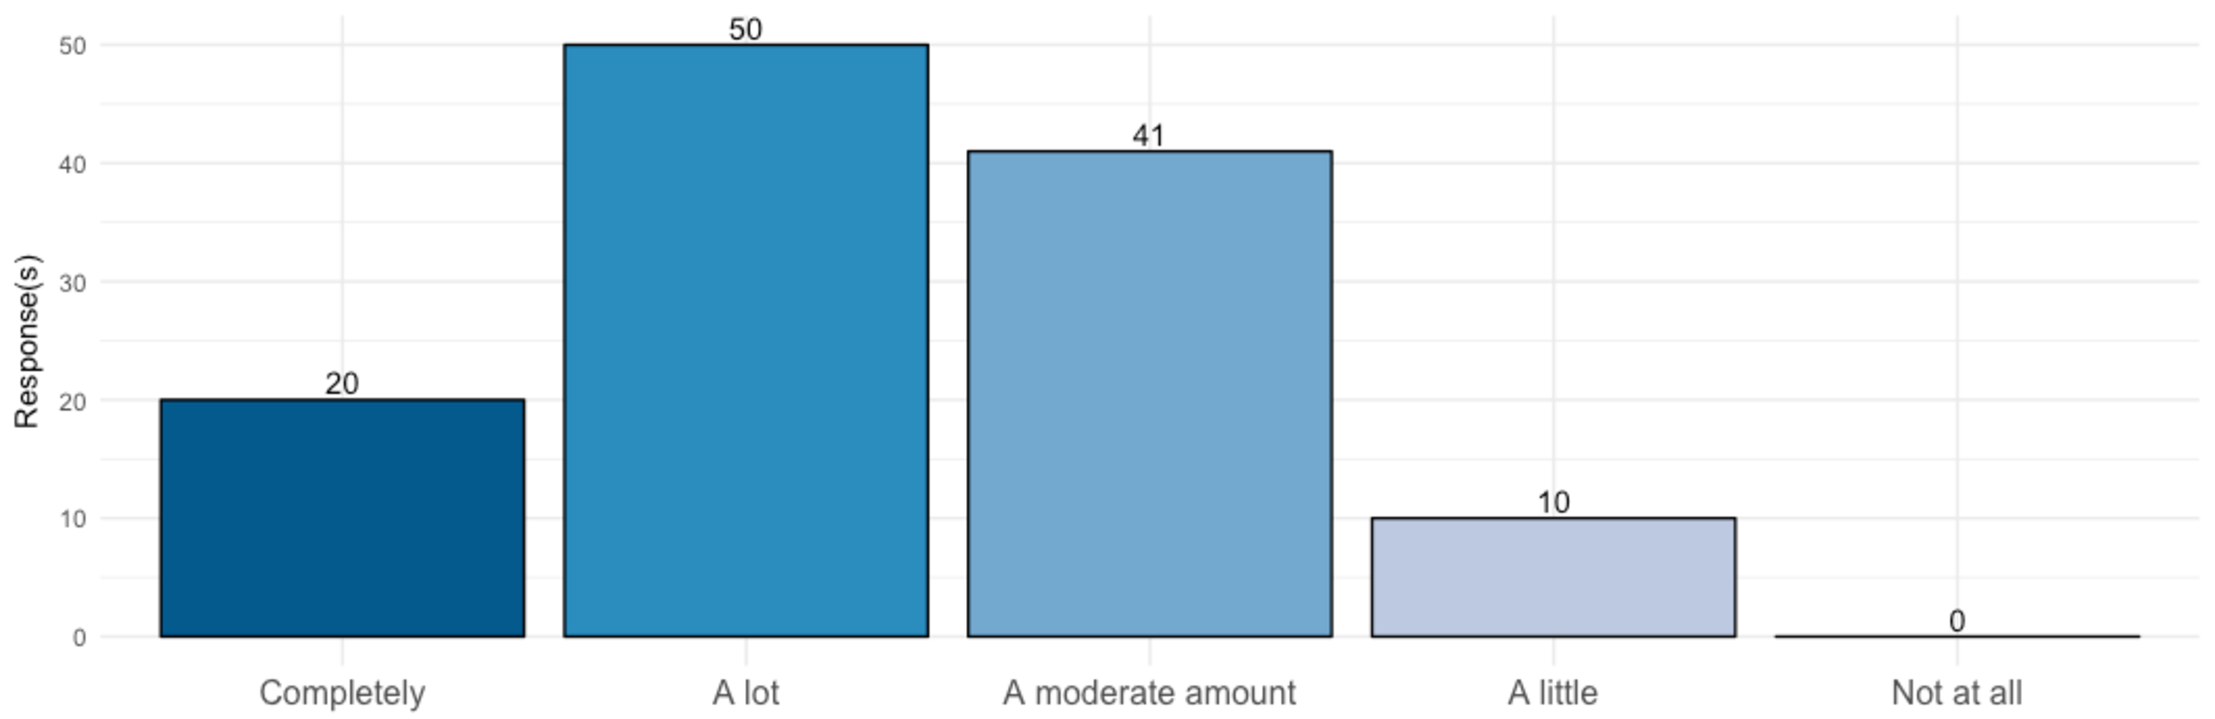
\includegraphics[width=0.95\textwidth,keepaspectratio]{s2_tool_trust}}
%	\caption{Degree of Trust for Merging, History Exploration, and Conflict Resolution Tools. Scale: 1 is \textit{completely} and 5 is \textit{not at all}. 121 out of 162 participants (74.69\%) provided a response to this question in the \textit{Barriers Survey}.\vspace*{-0.3\baselineskip}}
%	\label{fig:tool_trust}
%\end{figure}

\subsection{Perceptions of Tool Effectiveness}\label{tool_effectiveness}
The perceived size and complexity of merge conflicts affect the way in which developers plan, allocate, and enact resolutions.
To understand the degree to which these two factors impact developers' perceptions about the effectiveness of their toolsets, we asked \textit{Barriers Survey} participants to rate their toolset across four different merge conflict archetypes: (A1) \textit{simple, small merge conflicts}, (A2) \textit{simple, large merge conflicts}, (A3) \textit{complex, small merge conflicts}, and (A4) \textit{complex, large merge conflicts}.

\begin{figure*}[!htbp]
\centering
\fbox{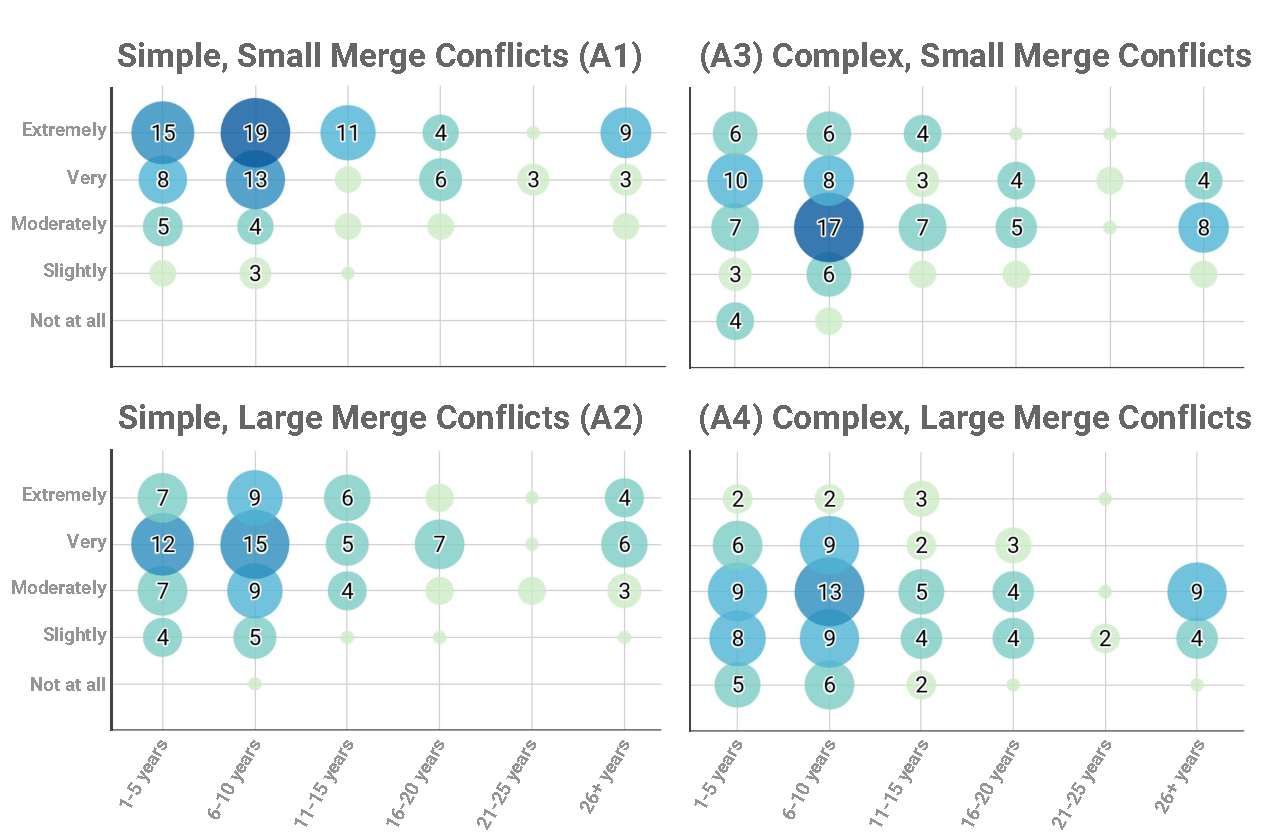
\includegraphics[width=0.98\textwidth,keepaspectratio]{BubbleChartUpdated.pdf}}
\caption{Effectiveness of developers' toolsets in supporting perceived size and complexity of merge conflicts, split on software development experience. Bubble values indicate number of \textit{Barriers Survey} responses for effectiveness of a particular merge conflict size and complexity, and bubble sizes indicate the number of responses for comparison.}
\label{size_vs_complexity}
\end{figure*}

%\begin{figure*}[!htbp]
%\centering
%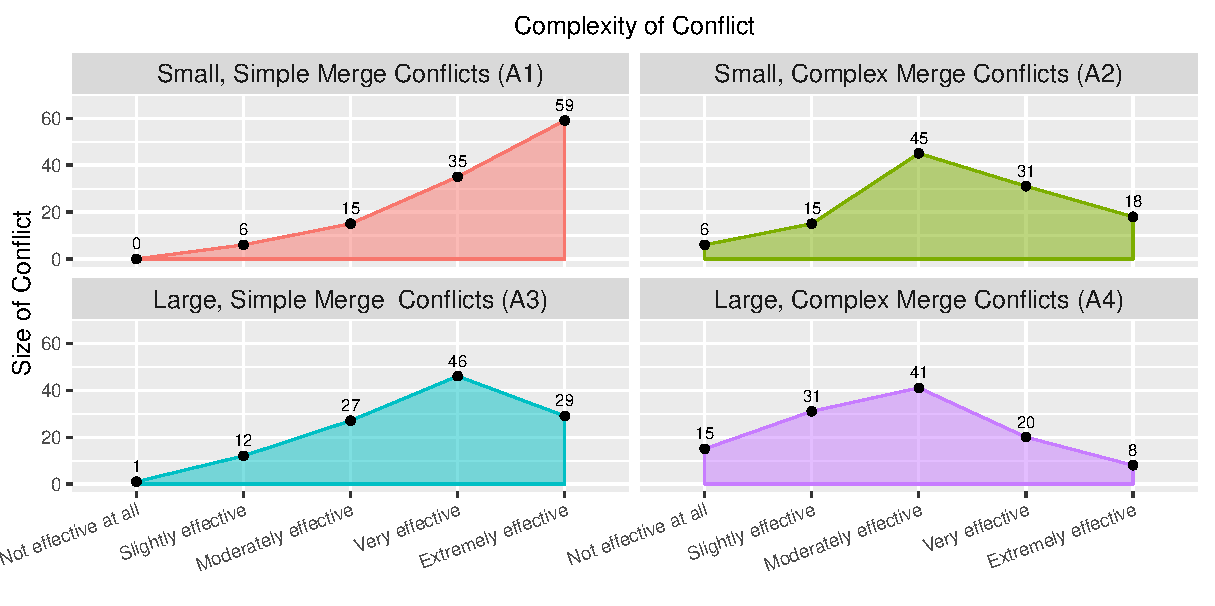
\includegraphics[width=1.01\textwidth]{ConflictComplexityVsSize.pdf}\vspace*{-1\baselineskip}
%\caption{Effectiveness of developers' toolsets in supporting perceived size and complexity of merge conflicts. Dot values indicate the number of \textit{Barriers Survey} responses for effectiveness of a particular merge conflict size and complexity, and the vertical height of each segment indicating the number of responses at each degree of effectiveness.\vspace*{-0.3\baselineskip}}
%\label{size_vs_complexity}
%\end{figure*}

Individual participants have different toolsets, and consider different factors when determining the perceived size and complexity of a merge conflict.
We therefore instructed participants to rate their own toolset using their notion of what constitutes \emph{simple} vs. \emph{complex} and \emph{small} vs. \emph{large} merge conflicts.

Figure~\ref{size_vs_complexity} provides a visual illustration of the results of this survey question.
The four plots display the results for each of the archetypes, with archetype (A1) in the top-left plot, (A2) in bottom-left plot, (A3) in the top-right plot, and (A4) in the bottom-right plot.
Individual plots are composed of a horizontal axis containing participants' software development experience, which we collect since experience can determine the range of conflicts that they have faced and their perceptions.
The vertical axis shows the range of possible responses for the effectiveness of merge toolsets.
The size and number within each bubble represent the number of respondents with a particular amount of software development experience that rated their toolset at that specific effectiveness level.

For example, a practitioner with 6-10 years of experience who indicates that her merge toolset is \textit{extremely effective} for \textit{small, simple merge conflicts} would be represented in the largest bubble (containing 19) in A1. % in the top-left plot. 
She would also be represented in the largest bubble (containing 13) in the bottom-right plot (A4) if she indicated that her merge toolset was \textit{moderately effective} for \textit{large, complex merge conflicts}.

Observing the overall trends when moving between plots, we find that developers perceive complexity of the conflict to have a greater impact on the effectiveness of their merge toolsets than the size of merge conflicts.
Numerical analysis confirms this when finding that the mean response for archetype (A1) is 4.278 (where 5 is \textit{extremely effective} and 1 is \textit{not effective at all}), (A2) is 3.782, (A3) is 3.347, and (A4) is 2.783.
The shift from \textit{small} to \textit{large} merge conflict size (A1 to A2) results in a difference in mean responses of 0.496, whereas the shift from \textit{simple} to \textit{complex} merge conflict complexity (A1 to A3) results in a difference in mean responses of 0.930.

Examining this trend through the lens of software development experience, we find that more experienced developers perceive a greater disparity in the effects of increasing merge conflict complexity (as opposed to merge conflict size) on the effectiveness of their merge toolsets.
Table~\ref{experience_vs_effectiveness} illustrates the numerical analysis between each of the software development experience groups defined in the \textit{Barriers Survey}.

\begin{table}[!htbp]
\renewcommand{\arraystretch}{1.2}
\caption{Mean effectiveness of developers' toolsets across software developer experience and merge conflict archetypes from \textit{Barriers Survey}}
\label{experience_vs_effectiveness}
\centering
\begin{tabularx}{\textwidth}{r|cccc|ccA{0.9cm}}
\toprule
  \rowcolor[gray]{0.85}
  \parnoteclear % tabularx will otherwise add each note thrice
  Experience\parnote{Software development experience of participants.} & A1\parnote{\label{mean_response}Mean response for the archetype; where 5 is \textit{extremely effective} and 1 is \textit{not effective at all}.} & A2\parnoteref{mean_response} & A3\parnoteref{mean_response} & A4\parnoteref{mean_response} & MC Size\parnote{Difference in mean responses when shifting from \textit{small} to \textit{large} merge conflict size (A1 to A2).} & MC Complexity\parnote{Difference in mean responses when shifting from \textit{simple} to \textit{complex} merge conflict complexity (A1 to A3).} & Diff.\parnote{Aggregate difference between MC Complexity and MC Size (negative indicates a reverse relationship).}\\
\midrule
  1-5 years & 4.200 & 3.733 & 3.367 & 2.733 & 0.467 & 0.833 & 0.367 \\
  \rowcolor[gray]{0.95}6-10 years & 4.231 & 3.667 & 3.256 & 2.795 & 0.564 & 0.974 & 0.410\\
  11-15 years & 4.438 & 4.000 & 3.563 & 3.000 & 0.438 & 0.875 & 0.438 \\
  \rowcolor[gray]{0.95}16-20 years & 4.167 & 3.833 & 3.333 & 2.750 & 0.333 & 0.833 & 0.500 \\
  21-25 years & 4.250 & 3.750 & 4.000 & 3.000 & 0.500 & 0.250 & -0.250 \\
  26+ years & 4.500 & 3.929 & 3.143 & 2.571 & 0.571 & 1.357 & 0.786 \\
\bottomrule
\end{tabularx}
\parnotes
\end{table}

When comparing the aggregate differences between shifting from \textit{small} to \textit{large} merge conflict size (A1 to A2) and shifting from \textit{simple} and \textit{complex} merge conflict complexity (A1 to A3), we see that participants with 1-5 years of software development experience have a 0.367 gap in dimensional differences (complexity vs. size mean differences).
This gap widens as the number of year of software development experience increases, until participants with 26+ years of software development experience have a 0.786 gap in dimensional differences.
The exception to this pattern is the small group of participants with 21-25 years of software development experience (10 participants, 4.42\% overall), who indicate that the size of a merge conflict has a greater impact on the effectiveness of their merge conflict toolsets.
We find that this group uses the same merge toolsets as the larger participant population (see Table~\ref{s2_toolset}), which suggests that concerns vary among experienced developers.

These results suggest that merge tools are currently equipped to handle increases in the size of merge conflicts, but not as well equipped for increases in complexity.
Additionally, more experienced developers perceive this gap to be greater than less experienced developers, suggesting that experienced developers have greater unmet needs for tool support when merge conflict complexity is unavoidable.
The increasing amount of code being developed in distributed environments means that scaling support in both dimensions is necessary to accommodate all developers' needs.
\section{Implications}\label{implications}

\subsection{For Developers}
Developers are in the middle of any situation involving merge conflicts, and the efforts required to resolve them.
Understanding the constraints that different phases of the merge conflict life-cycle place on time and resources can allow more effective prevention and management of any merge conflicts that do arise.

Developers indicate that understanding code, having appropriate information, and dealing with complex codesets are key themes of difficulty when working with merge conflicts (Sections~\ref{RQ1}, \ref{RQ2}).
Existing tool support can help with some of these issues, but developers also need to educate themselves on development processes that prevent and alleviate the severity of merge conflicts. 
For example, the number of conflicting files and the size of changes are considered important factors (Section~\ref{difficulty-factors}).
Researchers~\cite{brindescu2014versioncontrol} have previously found that developers using distributed version control systems commit more often, and that committing more often makes debugging easier when something breaks~\cite{meyer2014continuous}.
Therefore, developers should strive to make smaller commits, and commit often.

Other agile development processes such as continuous integration, iterative development, and branch merging policies are known to facilitate development in large, distributed teams. 
However, not all developers are actively using such techniques~\cite{phillips2011branching}, and large organizations will require additional diligence in order to address the increased possibility of conflicts occurring.
These organizations should strive to use proactive merge conflict monitoring and detection systems and processes, to speed up the transition from the \textit{awareness} and \textit{planning} phases and on through to the \textit{resolution} and \textit{evaluation} phases.

\subsection{For Tool Builders}
Version control systems provide an easy method for storing and retrieving recent development history, but examining older development history at scale and in a usable manner has not completely met developers' expectations.
Tool builders should work to address this unmet need by leveraging research in search systems for developer-assistance~\cite{nabi2016putting} and machine learning-based code assistance~\cite{bradley2011history_exploration} to provide intuitive and expressive tools for history exploration.

Even if developers use a \emph{reactive} monitoring approach for detecting merge conflicts, better tool support can make their lives easier.
For example, instead of notifying a developer that a merge conflict has occurred, adding an annotation within tools indicating the type of conflict might assist developers.
This type of contextualized information would allow developers to more precisely know how urgent the merge conflict is, without having to interrupt their workflow.

Developers indicate that current merge toolsets do not scale to handle large, complex merge conflicts (see Section~\ref{tool_effectiveness}).
To address this concern, tool builders should look at consolidating feature sets that currently span multiple tools in order to provide better usability (I1 from Table~\ref{s2_tool_improvements}).
Tool builders should also add more expressive search and filtering features for both project history and meta-information related to merge conflicts (I2, I3), to ease the frustration of developers that must understand the context and evolution of code involved in the conflict.

Before starting a merge conflict resolution, we found developers having to ``guess-timate'' the difficulty of the conflict resolution to decide whether to work on it now or deffer it, whether to integrate the changes or simply start over. 
Prediction tools that identify the complexity of conflicts and difficulty of resolution can help alleviate this.
This will provide to developers with enough information to make accurate and informed decisions in order to prevent further issues down the line.

When it comes to evaluating the result of a merge conflict resolution, we found that developers employ various strategies (Table~\ref{conditionsSuccess}).
Developers mentioned that passing tests (C1) and successful compilation (C2) are some of the criteria for success.
However, for large projects, running the test suite can be time intensive.
Tools can help developers by providing information or running only tests that are impacted by the conflict resolution.
This would help developers as they would have to rely less on their own intuition (C5), when it comes to evaluating the result.

\boldif{Conflicts might be difficult, because the result is hard to evaluate}
The fact that developers mention code complexity as one of the main factors in deferring a merge conflict resolution, and that developers ``eyeball'' the resolutions, seems to be an indication that evaluation might be a problem in the resolution.
Merge conflicts are perceived as difficult because \emph{the evaluation of the results are difficult.}
In this case, tools should provide better support for developers when they evaluate their resolution.

Finally, most developers have failed at least once in resolving a merge conflict resolution (Figure~\ref{fig:first-attempt-failure}).
Tools can provide better insight into why the resolution has failed, so developers have information to formulate their next steps.
Currently, when a merge conflict resolution fails, developers have to interrupt their workflow by taking the resolution offline (Table~\ref{backup-strategies}, B1), or they have to ask for help, which has the potential of interrupting other developers (B2).
If developers had more information about \emph{why} the merge conflict resolution failed, they might be able to recover more efficiently.

\subsection{For Researchers}
%Our results inform future research by providing insights into software developers' perspectives during merge conflicts.

The top factors that impact the assessment of merge conflict difficulty are primarily focused on program comprehension (F1, F3, F4 from Table~\ref{s2_factors}).
Program comprehension has been an important research focus, with entire conferences dedicated to it.
Previous research has explored tool support and visualizations to help comprehend programs, both small and large.
Our results indicate that developers still have unmet needs along the following dimensions: (1) comprehending code snippets in isolation, (2) understanding the code context underlying multiple code snippets that are split across multiple files, and commits, and; (3) the ability to quickly comprehend the complexity of these code snippets. 

%have a need to understand fragments of code, with some of this code split across multiples files, commits, or conflicting codebases.
%The ability to quickly evaluate the complexity of these code fragments is needed, including at the scale of text editors as evidenced by the use of basic toolsets instead of modern IDEs when working with merge conflicts (see Section~\ref{RQ3}).

Developers indicate that their needs during merge conflict resolutions center around the retrieval, organization, and presentation of relevant information (N1, N3, N4 from Table~\ref{s2_needs}).
With the variety of meta-information available across different toolsets, and the inconsistent use of terminology, there is a need for standardization and best practices to be developed.
Standardization efforts would likely help to alleviate some of the mistrust of merging tools that developers have expressed.
However, researchers should investigate the margin of errors that are tolerated by developers to determine the context in which developers discontinue use of tools.
 %threshold of merge tool errors that indicates whether a user will mistrust and discontinue use of those tools.

Expertise is seen as both a significant factor that affects the assessment of merge conflict difficulty (F2), and an important need for developers to effectively resolve the conflict (N2).
We have also seen that experience can play a part in developer's assessment of the success of a merge conflict resolution (C3).

Previous work has focused on recommending developers best suited to perform a collaborative merge based on the previous edits to conflicting files~\cite{dasilva2015niche} or developers' experience across branches and project history~\cite{CostaSarma}. 
However, these efforts have resulted in tools that require standalone installation and execution. 
Our results indicate that developers are concerned about toolset fragmentation, and therefore adding an additional tool might be counterproductive to the workflow of most developers. 

Our results show that 14 developers mention that they \emph{redo the changes} when a merge conflict resolution fails.
This \emph{Nuclear option} is very expensive.
Tools should provide better merging support, so developers can resolve a conflict and not have to scrap good code just because it happens to intersect with other changes.

Finally, we find that developers need to quickly estimate whether they can fix the conflict, and whether to resolve it now or delay the resolution. 
This indicates that developers need mechanisms to identify the skillsets required to complete the conflict resolution task, by viewing the code fragments (D1, D2).
Research should investigate mechanisms to identify required skillsets by using information retrieval or machine learning techniques on the code fragment and past edits.

\section{Threats to Validity}\label{threats}
As in any empirical study, there are threats to validity with our work.
We attempt to remove these threats where possible, and mitigate the effect when removal is not possible.

\paragraph{Construct Validity.}
Interview questions were open-ended and designed to elicit developer opinions about the experiences, difficulties, and perceptions of merge conflicts.
We determined particular factors and needs after concluding all interviews, and thus did not bias interview participants to only factors previously mentioned.
We created survey questions using factors found through card-based unitization.
This methodology allowed us to capture the common themes that developers experience when working with merge conflicts, but might have allowed themes specific to particular sub-groups to be unrepresented in our results.

\paragraph{Internal Validity.}
Confounding and extraneous factors can affect conclusions relating to cause and effect.
We lessen this effect by using multiple methods to triangulate our results, and compare against other datasets where appropriate.
Because we use these methods to highlight stronger answers, this also means that we may have missed subtle trends across our data that could have been visible otherwise.

\paragraph{External Validity.}
Interview results may not generalize to all developers due to a small sample size, but we reduce this effect by selecting interview participants from open- and closed-source projects, varying industries, and varying project sizes (see Table \ref{interview_demographics}).
To expand and confirm our interview results, we survey 102 and 162 developers on varying aspects to ensure our results match with trends in the larger software development community.
We do not report a response rate for our surveys, since social media and mailing lists do not allow accurate measurement of the number of individuals that read our recruitment message and did not choose to participate.


\section{Conclusion}\label{conclusion}
Practitioner perceptions of merge conflicts have an impact on their development process. First, they use perceptions to determine which tactics they will use to resolve the conflict.
After choosing how to resolve the conflict, practitioners encounter a new set of needs, both technical and social. 
Understanding these perceptions and needs is critical to understanding how to design tools which conform to the issues that these practitioners face in collaborative development.
We provide actionable implications for researchers, tool builders, and practitioners to harness the results of our study.
In future work, we hope to explore whether these factors, needs, and desired toolset improvements can be seamlessly merged into tools or techniques that assist developers' workflows.

%Merge conflicts interrupt development flow.
%Our work explores the human perceptions of merge conflict resolution in version control systems. We conducted an analysis of 10 interviews and confirmed our findings with a survey of 162 practitioners.
%
%We asked how practitioners approach merge conflicts and found that they identify 8 factors of importance for the initial evaluation of merge conflict difficulty. 
%We then asked which factors impact the difficulty of a merge conflict resolution and found 10 factors that impact the difficulty of the merge conflict resolution process. 
%These sets of factors serve as a way to inform managers and future research about merge-conflict-related difficulties of software practitioners.
%
%We also asked if developer tools met practitioner needs for merge conflict resolutions and found 6 improvements which practitioners would like to see in these tools. 
%In addition, we share specific tool needs from our interviews to give an idea of what people really struggle with in their merge conflict resolution workflows.
\section*{Acknowledgments}

We thank Iftekhar Ahmed, Amin Alipour, Alex Hoffer, Michael Hilton, Sruti Ragavan, and the anonymous reviewers for their valuable comments on earlier versions of this paper.
We also thank all of our interview and survey participants, especially those who helped distribute survey links.
This research was partially supported by NSF grants CCF-1439957, CCF-1553741, CCF-1560526, and IIS-1559657.


\bibliographystyle{spbasic}
\bibliography{Bibliography}

\end{document}


